\chapter{高频电外科发生器软件及控制系统设计}
\section{引言}
本文在第三章系统硬件系统设计的基础上，对高频电外科发生器系统的软件设计进行了详细介绍。基于IRF640N MOSFET和TC4420驱动芯片，本文所设计的推挽逆变电路如图\ref{inverter}所示。电路采用双管推挽结构，两个MOSFET分别连接在变压器初级线圈的两端，中心抽头连接可调直流稳压源输出电压。TC4420驱动芯片的输入端由MCU提供的PWM信号直接驱动，且通过适当的死区时间设置避免两个MOSFET同时导通引起的短路问题。
\section{高频采样信号检测与数字处理}
为了从采样电压电流信号中准确提取高频正弦波形的幅值及相位差，需要对ADC采集的离散数字信号进行分析和处理。常见的交流信号特征量分析方法可以从时域和频域两个层面实现。时域分析方法包括均方根法、正弦参数拟合法与正交解调法等，本质上是利用波形的几何或统计特征进行计算，实现过程直观且计算复杂度较低，但当采样信号中存在噪声或采样点未对准波峰、波谷时幅值估计精度容易受到影响，且部分方法在求取信号之间的相位关系时实现较为复杂。
频域分析方法则是将离散的时域采样信号投影到特定频率的基函数上，从而直接提取对应频率分量的频域响应，具有较好的频率选择性，并能有效抑制非目标频率成分和噪声对计算结果的影响。

本文系统的输出及采样信号频率均固定为350KHz，同时系统对交流信号的幅值和相位差信息精度要求较高，以提高有功功率和等效有功负载计算的准确度，因此本文采用频域分析方法对采样数据进行数字信号处理，整体可分为同步采样、频域分析、补偿校正以及数据拟合四个部分。具体处理流程如图\ref{signal_process}所示。
\begin{figure}[htbp]
	\centering
	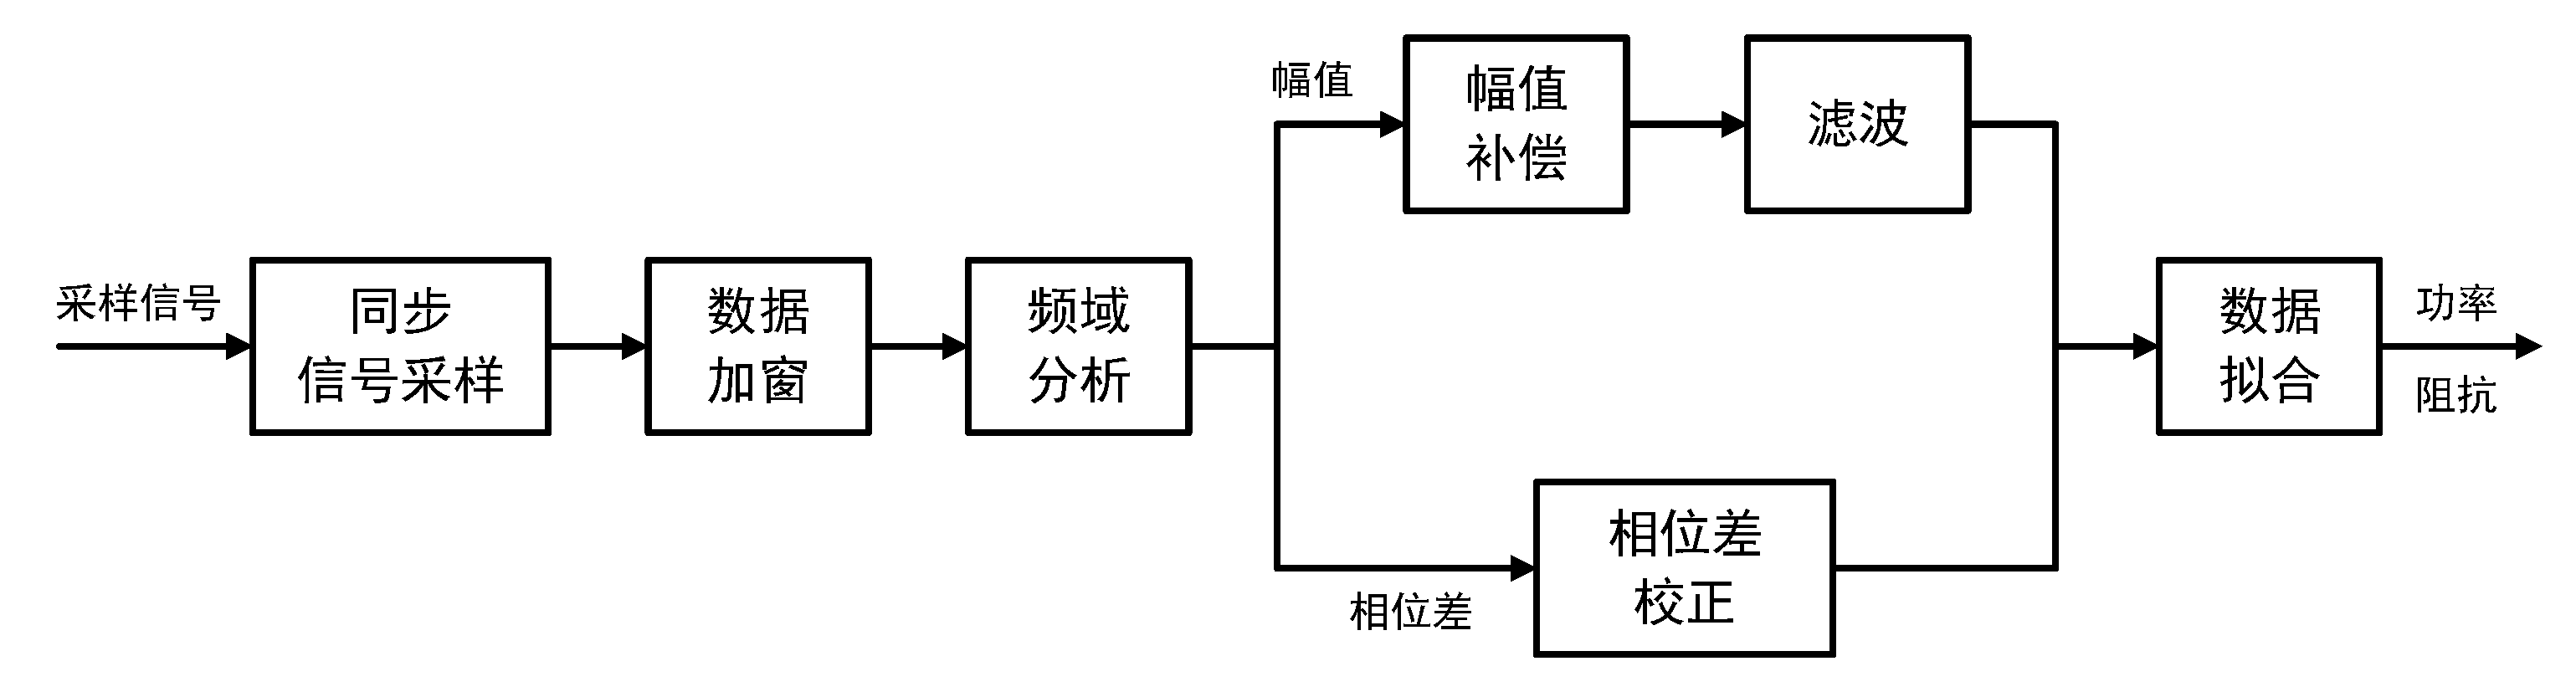
\includegraphics[scale=0.318]{Fig/signal_process.pdf}
	\caption{\label{signal_process}高频采样信号数字处理流程图}
\end{figure}

\subsection{Goertzel算法}
对于有限长度的离散采样序列，常用的频域分析方法是离散傅里叶变换（DFT），其基本思想是将输入序列表示为若干离散复指数基函数的线性组合，由于这些基函数在有限长度区间内满足正交性，因此可通过内积运算求得测量信号在各个离散频率分量上的响应强度。DFT的数学定义为：
\begin{equation}
	X[k] = \sum_{n=0}^{N-1} x[n] e^{-j\frac{2\pi}{N} kn} = \sum_{n=0}^{N-1} x[n] W_N^{kn}, k=0,1,...,N-1  \label{dft}
\end{equation}
其中$x[n]$为输入的时域采样序列，$N$为离散信号点数，$X[k]$表示序列在第k个离散频率点上的频域响应，$W_N^{k}$为旋转因子。由式(\ref{dft})所示，DFT计算结果包含N个离散频谱样本，每个频点对应的实际频率为$f_k = kf_s/N$，其中$f_s$为采样频率，由此可见在采样频率固定的情况下采样点数N越大，频率分辨率越高，从而能够区分更加接近的频率成分，但同时也意味着更长的数据观测窗口以及更大的计算开销，在实际应用中需要在分析精度与实时性之间进行权衡。

对于实值信号，DFT获得的频谱具有共轭对称性，即$X[N-k] = X^*[k]$，因此通常只需分析前半部分频谱即可获得主要频率信息。对于频谱值$x_k$，由于复指数形式的旋转因子可以表示为正弦项与余弦项的组合，每个频谱复数值可进一步计算出输入信号在对应频率上的幅值和相位信息，如式(\ref{amp_phase})所示：
\begin{equation}
	\begin{cases}
		e^{-j \frac{2 \pi} {N} k n}=W_N^{kn} = \operatorname{c o s} \left( \frac{2 \pi} {N} k n \right)-j \operatorname{s i n} \left( \frac{2 \pi} {N} k n \right) \\
		\left| X [ k ] \right| = \sqrt{Re(X[k])^2 + Im(X[k])^2}, \angle X [ k ] = arctan\left(\frac{Im(X[k])}{Re(X[k])}\right)  \label{amp_phase}
	\end{cases}
\end{equation}

根据DFT的定义式可得，计算单个频点的频谱值通常需要约N次复数乘法和N−1次复数加法，完整的N点DFT计算复杂度为$O(N^2)$。快速傅里叶变换算法（FFT）对DFT中大量重复计算过程进行了优化，采用分治策略将N点DFT分解为多个更短序列的DFT计算，并利用旋转因子的周期性对结果进行合并，从而将计算复杂度降低至$O(N \log N)$，显著提高了大规模频域分析的效率。
然而FFT算法对于信号序列长度具有一定要求，例如基2 FFT需要采样点数满足$N=2^m$，以便进行递归分解和蝶形运算，当采样点数不符合特定快速分解结构时，FFT的算法运算效率和实现复杂度将会下降。

DFT在分析有限长序列时隐含地默认原始采样数据在时间轴上按长度N周期延拓，若输入信号在采样窗口内不是整数周期，其周期延拓后的序列在在窗口边界处通常会出现不连续现象，在频域上表现为频谱能量向邻近频率点扩散，产生频谱泄漏现象，从而降低目标频率处幅值估计的准确性。因此在基于DFT进行频谱分析时，需要合理设计采样频率$f_s$与采样点数$N$，使目标信号频率尽可能对应于离散频谱中的整数频点。

在本文系统中仅需关注350KHz频率成分，而FFT算法所需采样点数与ADC采样频率组合难以保证目标频率恰好落在频谱整数点上。因此本文选择采用适用于单频或少数频点检测场景Goertzel算法进行频域分析。

Goertzel算法是一种针对指定频率分量进行递推计算的高效算法，核心思想是通过一个二阶递推结构计算输入序列与目标频率基函数的内积，从而直接得到该频率分量的幅值和相位信息。若目标频点在离散频谱上的索引为K，构造递推输出序列$y[n]$，并使用$y[n]$表示K点处的DFT频谱值$X[K]$，则有：
\begin{equation}
	\begin{cases}
		y[n] = y[n-1] e^{j 2 \pi \frac{K}{N} } + x[n] \\
		X[K] = y[N-1]e^{j2\pi\frac{K}{N}}       \label{goertzel:1}
	\end{cases}
\end{equation}
对输出序列$y[n]$进行z变换，可得到其与输入序列$x[n]$的系统函数关系为：
\begin{equation}
	\frac{Y ( z )} {X ( z )}=(1-e^{-j 2 \pi\frac{K} {N}} z^{-1})\cdot\frac{1} {1-2 \operatorname{c o s} \left( 2 \pi\frac{K} {N} \right) z^{-1}+z^{-2}} = \frac{Y ( z )} {S ( z )} \cdot \frac{S ( z )} {X ( z )}
\end{equation}
其中$S(z)$为所设中间状态变量$s[n]$的z变换，对$\frac{S ( z )} {X ( z )}$进行z反变换可得递推关系为：
\begin{equation}
	s[n] = x[n] + 2 \cos \left( \frac{2 \pi K} {N} \right) s[n-1] - s[n-2] \label{goertzel:3}
\end{equation}
其中初始条件为$s[-1] = 0, s[-2] = 0$。该式可视为输入序列通过一个二阶无限脉冲响应（IIR）滤波器后得到状态变量$s[n]$输出，滤波器的极点位于单位圆上与目标频率对应的位置，因此对该频率附近的输入信号分量具有较强响应。对$\frac{Y ( z )} {S ( z )}$进行z反变换可得：
\begin{equation}
	y[n] = s[n] - e^{-j 2 \pi\frac{K} {N}}s[n-1]    \label{goertzel:2}
\end{equation}
该过程可视为有限脉冲响应（FIR）滤波器，在系统函数中引入一个零点，对内部状态进行相位校正与输出映射。将式(\ref{goertzel:2})代入式(\ref{goertzel:1})中，可得该频点处的频谱信息为：
\begin{equation}
	\begin{gathered}
		X[K] = e^{j \frac{2 \pi K} {N}}s[N-1] -  s[N-2] \label{goertzel:4}  \\
		\begin{cases}
			| X [ K ] |=\sqrt{\left( \operatorname{c o s} (\frac{2 \pi K} {N})s [ N-1 ]- \, s [ N-2 ] \right)^{2}+\left( \operatorname{s i n} (\frac{2 \pi K} {N}) \, s [ N-1 ] \right)^{2}} \\
			\angle X [ K ]=\operatorname{a r c t a n} \cfrac{\operatorname{s i n} (\frac{2 \pi K} {N}) \, s [ N-1 ]} {\operatorname{c o s} (\frac{2 \pi K} {N})s [ N-1 ]- \, s [ N-2 ]}
		\end{cases}
	\end{gathered}
\end{equation}
式(\ref{goertzel:3})和式(\ref{goertzel:4})导出的Goertzel 算法信号流图如图\ref{goertzel_chart}所示：
\begin{figure}[htbp]
	\centering
	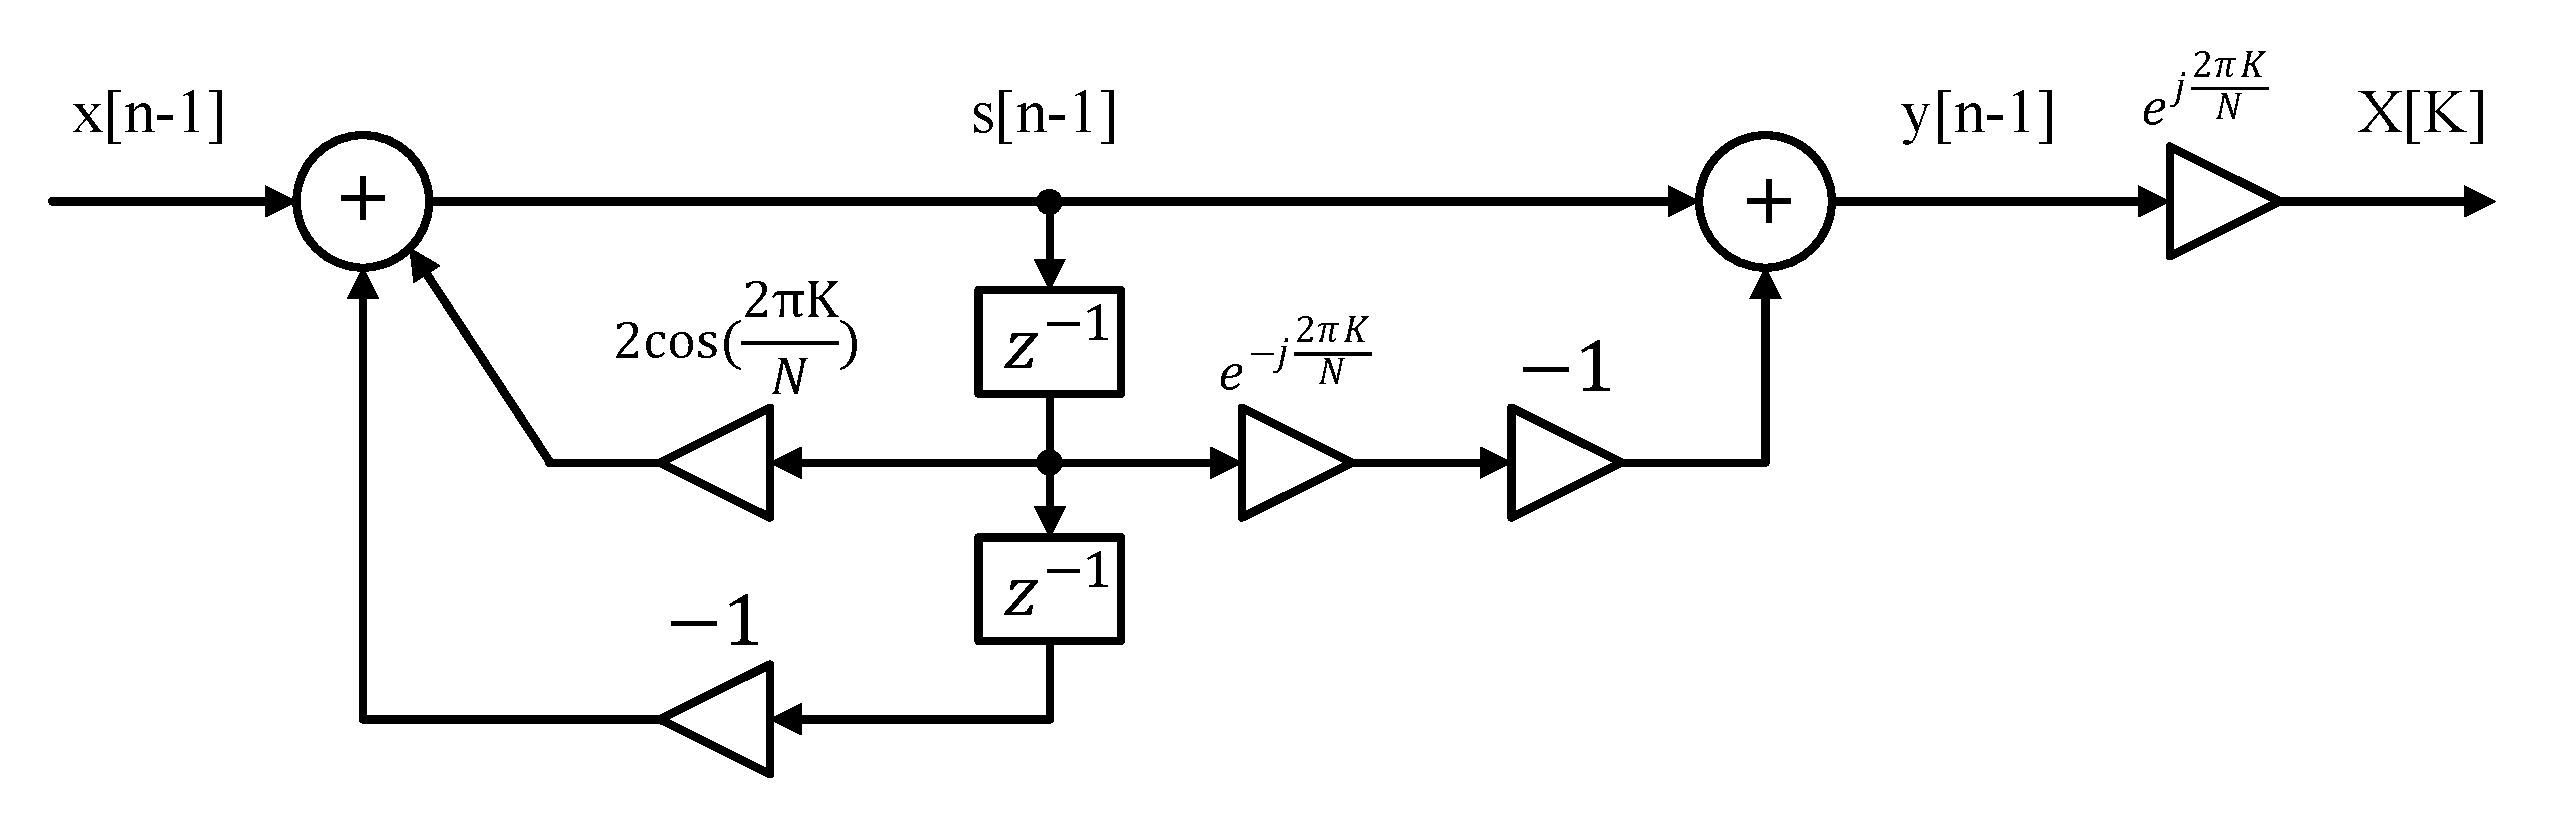
\includegraphics[scale=0.35]{Fig/goertzel_chart.pdf}
	\caption{\label{goertzel_chart}Goertzel算法信号流图}
\end{figure}

在固定频率信号检测场景中，Goertzel算法仅包含实数乘法、加法以及少量三角函数计算，保持较高的计算效率的同时不受到采样点数选取的限制，同时其递推结构的程序实现简单，适合资源和性能受限的嵌入式微控制器平台。在STM32F303VCT6硬件平台上测试三种频域分析算法的运行耗时如表\ref{efficence}所示。
\begin{table}[htbp]
	\caption{\label{efficence}微控制器频域分析算法运行耗时对比}
	\centering
	\small
	\setlength{\tabcolsep}{10pt}
	\begin{tabular}{c c c c }
		\hline
		频域分析算法 & FFT（DSP优化） & 单频点DFT  & 单频点Goertzel \\
		\hline
		计算耗时   & 2.95ms     & 0.766ms & 0.234ms     \\
		\hline
	\end{tabular}
\end{table}
结果表明，尽管FFT算法在计算过时经过DSP库的加速优化，但由于包含全部频谱仍然需要较长时间；单频点DFT的计算量虽然减小，但仍然需要逐点进行复数运算；相比之下，Goertzel算法在单一频率检测场景下具有更高的运算效率，因此本文最终选用Goertzel算法对高频输出采样信号进行频谱分析。该算法在微控制器中的实现伪代码如列表\ref{goertzel_code}所示。
\begin{algorithm}
	\caption{Goertzel算法实现伪代码}
	\label{goertzel_code}
	\begin{algorithmic}[1]
		\setlength{\baselineskip}{16pt} % 设置伪代码行间距
		\State \textbf{Input:} sample\_data[N], K
		\State $\text{s\_prev} \gets 0$, $\text{s\_prev2} \gets 0$, $\text{s\_curr} \gets 0$
		\State $\text{real} \gets 0$, $\text{imag} \gets 0$
		\State $\text{cosine} \gets \text{cos(2πK/N)}, \text{sine} \gets \text{sin(2πK/N)}$
		\State $\text{index} \gets 0$
		\While{$\text{index} < N$}
		\State $\text{s\_curr} \gets \text{sample\_data[index]} + 2\cdot \text{cosine} \cdot \text{s\_prev} - \text{s\_prev2}$
		\State $\text{s\_prev2} \gets \text{s\_prev}$
		\State $\text{s\_prev} \gets \text{s\_curr}$
		\State $\text{index} \gets \text{index} + 1$
		\EndWhile
		\State $\text{real} \gets \text{cosine} \cdot \text{s\_prev} - \text{s\_prev2}, \text{imag} \gets \text{sine} \cdot \text{s\_prev}$
		\State \textbf{Output:} real, imag
	\end{algorithmic}
\end{algorithm}

\subsection{同步信号采样}
根据前述频域算法的特点，需合理选取ADC的采样频率和采样点数，使目标信号频率尽可能落在离散频谱的整数频点上。在STM32微控制器内部集成的ADC中，采样位数越低单次转换时间越短，从而可以实现更高的采样频率。综合系统对电压电流信号分辨率的需求，本文选择ADC工作在10位分辨率模式，该分辨率下系统最大输出电压采样误差为$\frac{316.2V}{2^{10}}\approx 0.31V$，采样误差可控制在容许范围之内。根据所选芯片的数据手册，ADC时钟频率为72MHz，10位分辨率完成单次转换需要10.5个ADC时钟周期，而ADC的采样时间则由软件配置，且仅提供若干离散档位，因此无法任意设定采样频率。在上述约束条件下，采样点数$N$可表示为：
\begin{equation}
	N = \frac{k \cdot f_s}{350KHz} = \frac{k \cdot 72MHz}{350KHz \cdot (T_{conv}+10.5 )}, T_{conv}= 1.5,2.5,...,601.5, k \in\mathbb{Z}^{+} \label{sample_num}
\end{equation}
经综合权衡本文最终选择采样时间为19.5个ADC时钟周期，外部采样电路可满足对于输入阻抗的需求，此时采样频率为2.4MHz。取采样点数为1022点，目标频率350KHz在离散频谱中接近整数频点位置$\frac{350KHz \cdot 1022}{2.4MHz} = 149.04$。

由2.3节对生物组织阻抗特性的分析可知，系统负载阻抗通常呈现阻容特性，而实际作用于人体组织的能量为系统输出的有功功率。因此需要通过频域分析方法提取输出电压电流信号的相位差，以实现有功功率以及等效阻抗的精确计算。为保证相位计算的准确性，高频输出信号的采样过程必须保持同步。通过在PCB布局中对采样信号进行等长布线，电压与电流信号能够同步到达微控制器的输入端，而在ADC采集过程也需保持同步采样才能减少相位信息计算误差。本系统中分别使用两个独立的ADC外设对电压与电流信号进行采样并工作在连续转换模式下，同步采样方案如图\ref{sync_sample}所示。
\begin{figure}[htbp]
	\centering
	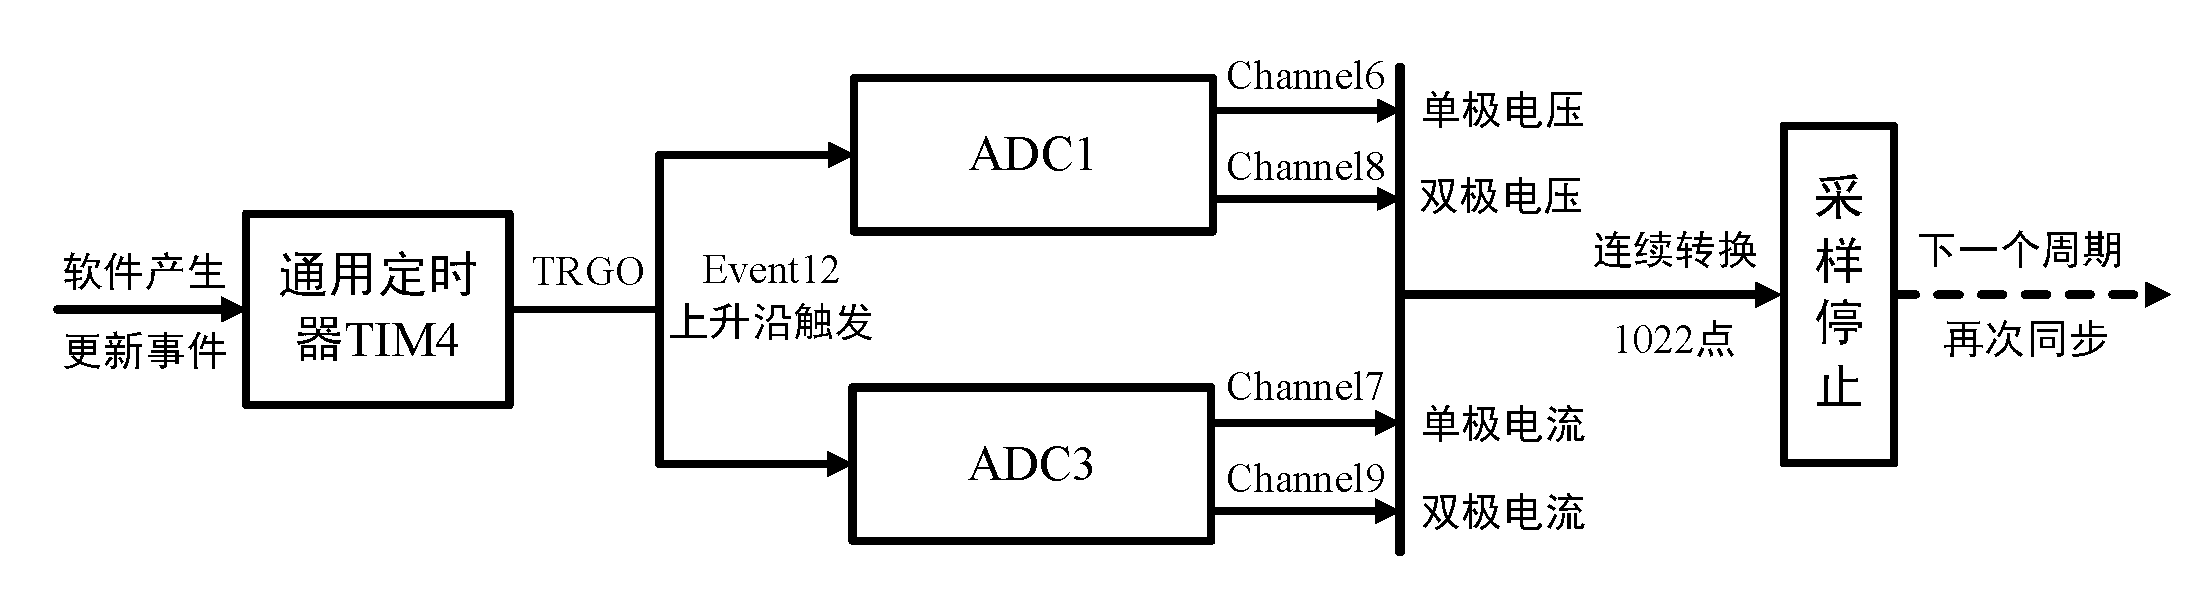
\includegraphics[scale=0.44]{Fig/sync_sample.pdf}
	\caption{\label{sync_sample}电压电流同步采样示意图}
\end{figure}

由上图可知，ADC的外部触发源设为event12，该触发信号由STM32内部通用定时器的TRGO输出产生。TRGO信号是定时器用于触发内部其他外设的专用信号，其触发源可设置为计数器复位事件或比较事件等，本系统选择计数器更新事件作为触发源。
为了使同步采样的触发时刻更加可控，本文采用仅使能定时器但不启动计数的软件触发方式，在特定的程序流位置产生更新事件。触发同步采样后，两路ADC连续转换1022点电压电流信号后在中断服务程序中停止ADC转换过程，并在下一个控制周期重新触发同步采样，以避免长时间连续转换产生的相位误差积累。

\subsection{频域分析及数据处理}
获取采样数据后，通过Goertzel频域分析算法计算目标频率分量的幅值和相位信息。然而前文所述采样频率和采样点数的选择并未使目标频率严格对应于整数频点，同时能量发生电路和采样电路也会引入微小的频率偏移，频谱泄漏现象难以避免。为了进一步提高频域分析计算结果的准确性，本文在算法处理之前先对采样数据进行加窗处理。窗函数的本质是对截取数据进行平滑加权，从而减弱时域序列截断边界处的不连续性。常见窗函数包括汉宁窗、海明窗等，与直接截断对应的矩形窗相比，这些窗函数在频谱上的旁瓣电平更低，抑制目标频率能量向邻近频点扩散，但其代价为主瓣宽度增大，导致频率分辨率下降。常见窗函数的时域波形及频谱特性如图\ref{window}所示。
\begin{figure}[htbp]
	\centering
	\subfloat[时域波形]{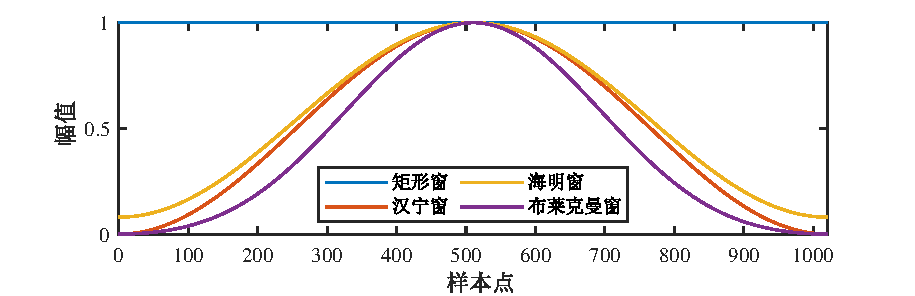
\includegraphics[scale=1]{MATLAB_plot_files/window_t.pdf}%
		\label{time}} \\
	\subfloat[单边频谱特性]{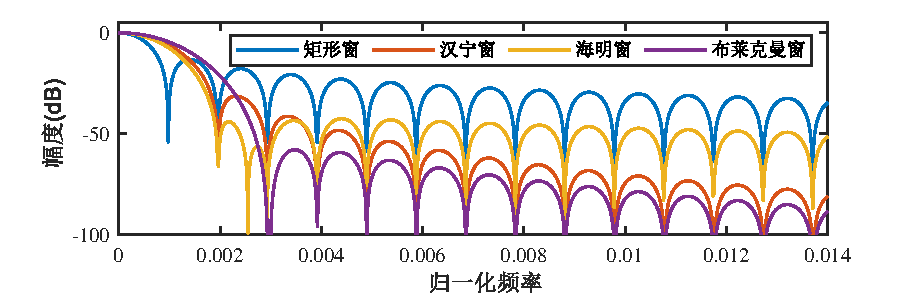
\includegraphics[scale=1]{MATLAB_plot_files/window_f.pdf}
		\label{frequency}} \\
	\caption{常见窗函数的时域波形及频谱特性}   \label{window}
\end{figure}

窗函数的选择需要在频率分辨能力和泄露抑制能力之间进行权衡。由于本系统目标信号频率较为单一，且对频谱分析的准确性要求较高，因此选择具有较好旁瓣抑制能力的汉宁窗进行数据加权处理。汉宁窗是一种实值余弦窗函数，其函数$w[n]$定义为：
\begin{equation}
	w[n] = 0.5 \cdot \left( 1 - \operatorname{c o s} \frac{2 \pi n} {N-1} \right), n=0,1,...,N-1
\end{equation}
该窗函数在时域上关于中心对称，对序列中间样本赋予较高权重，首尾部分逐渐衰减为零。汉宁窗在计算过程中包含余弦运算，若在每次对采样数据加窗时在线计算余弦系数将会增加微控制器的运算负担，为此本文采用以存储空间换取运算时间的方式，预先离线计算长度为1022点的汉宁窗系数，以数组的形式存储于微控制器的Flash中，按索引依次读取相应的窗系数对数据进行加权处理，提高系统整体的实时处理能力。

加窗后的采样序列通过Goertzel算法得到的幅值并不直接等于ADC采样信号的实际幅值，而是同时受到频谱特性以及加窗缩放的共同影响，因此还需对计算结果进行相应的幅值补偿。对于实值单频正弦信号，其频谱满足共轭对称性，当目标频率对应频点不位于奈奎斯特频点时，频域分析算法所得为单边频谱正频率分量响应，幅值仅占时域输入信号实际幅值的一半，因此首先需要进行双边频谱对称性补偿。其次，由于窗函数的引入改变了信号的整体幅值尺度，其系数的加权作用会使频谱分量的幅值发生缩放，还需对此缩放部分进行补偿。总幅值补偿公式可表示为：
\begin{equation}
	% A = \frac{2 \cdot |X[K]|} {N \cdot \overline{w}}
	A = \frac{2 \cdot |X[K]|} {\sum_{n=0}^{N-1} w [ n ]}  = \frac{2|X[K]|}{510.5}
\end{equation}
其中，$|X[K]|$为目标频率单边频谱幅值，$\sum_{n=0}^{N-1} w [ n ]$为窗函数加权系数的总和。通过上述补偿处理后，系统能够更加准确地恢复采样信号的真实幅值。

在微控制器的在线调试模式下通过脚本文件导出运行时SRAM数组内保存的1022点ADC采样电流数据，并导入到MATLAB环境中对该序列进行汉宁窗函数加权处理，绘制的数据波形如图\ref{samp_result}所示。
\begin{figure}[htbp]
	\centering
	\subfloat[前50点原始采样数据]{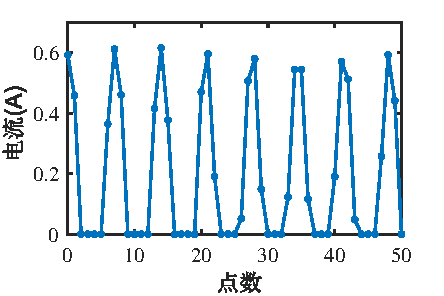
\includegraphics[scale=1]{MATLAB_plot_files/samp_volcur.pdf}}%}
	\subfloat[前50点加汉宁窗后的采样数据]{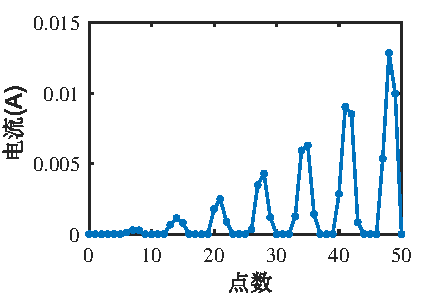
\includegraphics[scale=1]{MATLAB_plot_files/samp_volcur_win.pdf}}
	\caption{原始数据与加窗后数据对比}  \label{samp_result}
\end{figure}
由采样数据的时域波形可知，微控制器ADC输入结构会对交流的正弦信号进行半波整流。与此同时采样序列加窗后整体波形幅值发生一定程度的缩放，并且在序列的首尾部分衰减为零，与汉宁窗的时域特性相符。半波整流效应的引入会对采样信号的频谱结构产生一定的影响。若原始输入的正弦信号表示为$x_1(t)=A \operatorname{s i n} ( \omega t )$，则经过半波整流后的信号$x_1(t)$的傅里叶级数为：
\begin{equation}
	% x_{2} ( t ) = \left\{
	% \begin{array}{ll}
	%     A \operatorname{s i n} ( \omega t ), & 0 \leq t < \pi / \omega \\
	%     0, & \pi / \omega \leq t < 2 \pi / \omega
	% \end{array}
	% \right.
	x_{2} ( t )=\frac{A} {\pi}+\frac{A} {2} \sin( \omega t )-\frac{2 A} {\pi} \sum_{n=1}^{\infty} \frac{\cos( 2 n \omega t )} {4 n^{2}-1}   \label{half_wave_rectification}
\end{equation}

式(\ref{half_wave_rectification})表明半波整流后的信号在频谱中基频分量的幅值变为原始信号的一半，同时信号出现直流分量及偶次谐波分量，在频谱上表现为额外的谱线分布。由于本文仅对单一频点350KHz处的频谱分量进行提取，输入钳位产生的谐波分量均远离目标频点，可忽略频谱泄露导致频率分量之间的干扰，因此仅需在幅值补偿部分额外引入钳位导致基频分量幅值减半的修正。对1022点电流采样数据进行FFT频域分析并进行幅值补偿，得到加窗前后的单边频谱结果如图\ref{FFT_result}所示。
\begin{figure}[htbp]
	\centering
	\subfloat[原始采样数据频谱]{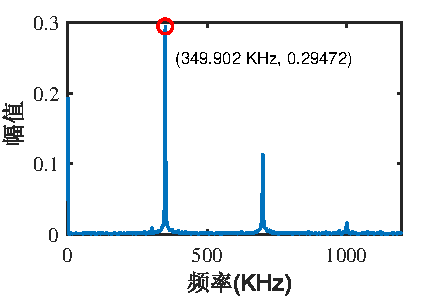
\includegraphics[scale=1]{MATLAB_plot_files/samp_volcur_fft.pdf}}%}
	\subfloat[加汉宁窗后采样数据频谱]{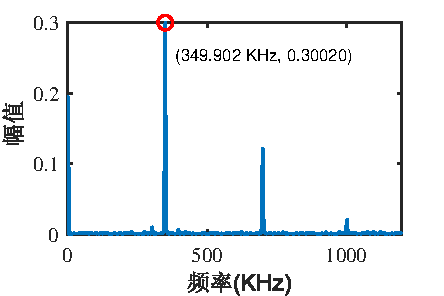
\includegraphics[scale=1]{MATLAB_plot_files/samp_volcur_win_fft.pdf}  \label{FFT_result_win}}
	\caption{原始数据与加窗后数据频谱对比}\label{FFT_result}
\end{figure}

从图中可以看出，采样数据频谱中出现了额外频率分量的谱线，与式(\ref{half_wave_rectification})的理论分析结果一致。频谱峰值主要集中在目标频点149处，未加窗时该频点附近存在一定程度的能量扩散；而经过汉宁窗加权处理后，目标频点的频谱能量更加集中，主要谐波分量在邻近频点的能量扩散均得到抑制。由于本文目标频点已经接近离散频谱的整数点，因此频谱泄漏本身较小，窗函数带来的改善相对有限。
进一步在Matlab环境中实现Goertzel算法，并对同一组电流采样数据进行计算，可得149频点处的幅值结果为0.3002，与图\ref{FFT_result_win}中FFT计算结果一致。上述实验结果表明，结合加窗与幅值补偿的Goertzel算法能够在实际硬件平台的采样数据上准确计算目标频率分量的幅值。

为减小多帧采样时频域响应因采样噪声及负载扰动等因素产生的波动，提高闭环控制反馈量的平稳度，本文在幅值补偿的基础之上通过一阶IIR低通滤波器对幅值计算结果进行平滑处理。该数字滤波器的差分方程表示为：
\begin{equation}
	y[n] = \alpha x[n] + (1-\alpha) y[n-1]
\end{equation}
其中$x[n]$为当前采样帧计算幅值，$y[n]$为滤波器输出，$\alpha$为滤波系数。滤波系数$\alpha$决定了滤波器的动态特性，$\alpha$较小时输出变化更加平滑，同时也会增加系统的响应时间；$\alpha$较大时输出快速跟随实际变化，但对噪声的抑制效果较差。考虑到本文采样帧与幅值计算的频率较高，且闭环控制目标侧重于反馈量的平稳变化，因此最终选择滤波系数$\alpha = 0.3$，实验结果证明具有较好的滤波和控制效果。

上述方法主要总结了频域分析计算幅值的补偿与滤波处理机制。对于采样信号的相位差信息而言，汉宁窗引入会在频率响应中包含与窗中心位置相关的固定线性相移，不会产生额外的非线性相位畸变。由于电压电流信号采样点数相同、采样时刻同步并使用相同的信号处理算法，该线性相移在双通道相位差计算过程中会相互抵消。然而实际系统中相位差计算准确度还会受到采样测量链路以及电流间接采样方式的共同影响，因此仍需通过实验标定的方式对相位差计算结果进行校正。相位差的修正关系可表示为：
\begin{equation}
	\phi_{\mathrm{t r u e}}=\phi_{\mathrm{a l g}}-\Delta\phi_{\mathrm{c h a i n}}+\Delta\phi_{C}
\end{equation}
其中$\phi_{\mathrm{a l g}}$为频域分析计算相位差，$\Delta\phi_{\mathrm{c h a i n}}$为采样测量链路相位补偿量，$\Delta\phi_{C}$为测量方式引入的相位修正量。采样链路中的附加相移通常由采样电路器件差异与寄生参数等因素引入，因此在校正时通过示波器同时测量系统高频输出信号的实际相位关系，与算法结果$\phi_{\mathrm{a l g}}$进行比较，其固定差值作为$\Delta\phi_{\mathrm{c h a i n}}$加入补偿，实验测得该补偿量约为0.279rad。其次，如前文3.5章所述，本文并未直接采样电流信号，而是通过采样高频电流流经采样电容两端电压间接获取电流信息，$\phi_{\mathrm{a l g}}$实际反映的是负载电压与采样电容电压之间的相位关系，因此需要对采样电容引入的相移进行补偿。在校正时使用阻抗分析仪UC8050L测量采样电容在目标工作频率处的实际阻抗相位，将其作为$\Delta\phi_{C}$叠加至$\phi_{\mathrm{a l g}}$，实验测得该补偿量约为1.56474rad。

为验证相位差计算及补偿处理的准确性，本文在两种典型负载条件下进行了实验测试：一类为纯电阻负载，另一类为阻容复合负载。实验过程中，使用频域分析算法计算并校正相位差与阻抗分析仪测量负载的相位关系进行对比，其结果如图()所示。

\begin{figure}[htbp]
	\centering
	\subfloat[电压采样数据拟合]{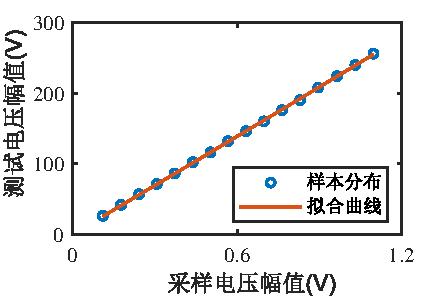
\includegraphics[scale=1]{MATLAB_plot_files/outputfit_vol.pdf}}%}
	\subfloat[电流采样数据拟合]{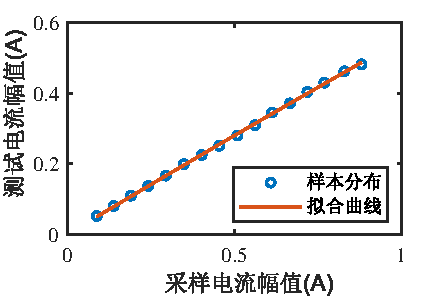
\includegraphics[scale=1]{MATLAB_plot_files/outputfit_cur.pdf}}%}
	\caption{最小二乘法数据拟合结果}
\end{figure}

实验结果表明，在纯电阻与阻容负载条件下，计算结果与阻抗分析仪测量结果之间的误差较小，证明校正环节能够有效消除采样链路与测量方式带来的附加相移，最终得到的相位差能够更准确地表征负载电压与实际输出电流之间的真实相位关系。

上述信号处理流程完成后，系统仍需将计算得到的采样信号幅值恢复为实际输出信号幅值。对于电压电流采样电路，需结合电阻网络阻值及采样电容的容值计算，还需考虑器件参数误差以及寄生参数的影响。为了提高幅值计算结果的准确性，本文采用最小二乘法对实际输出数据进行二次拟合。设通过示波器测量的实际输出信号幅值为${Y}$，由采样信号幅值组成的系数矩阵为$X$，拟合参数向量为$A$，拟合目标为求得最佳参数使得采样与实际信号之间残差平方和最小$\operatorname* {m i n}_{A} \Vert Y-X A \Vert_{2}^{2}$。最小二乘的正规方程解为：
\begin{equation}
	\begin{gathered}
		A = (X^T X)^{-1} X^T Y  \\
		\text{其中}:
		\renewcommand{\arraystretch}{0.85}       %控制间距
		X=\left[ \begin{matrix} {{x_{1}}^{2}} & {{x_{1}}} \\ {{x_{2}}^{2}} & {{x_{2}}} \\ {\vdots} & {\vdots} \\ {{x_{m}}^{2}} & {{x_{m}}} \\ \end{matrix} \right], \quad Y=\left[ \begin{matrix} {{y_{1}}} \\ {{y_{2}}} \\ {\vdots} \\ {{y_{m}}} \\ \end{matrix} \right],\quad A=\left[ \begin{matrix} {a_{1}} \\ {a_{2}} \\ \end{matrix} \right]
	\end{gathered}  \label{least_square}
\end{equation}
式中，$X$矩阵相比范德蒙矩阵减少了常数项，从而确保拟合函数能够经过原点。将输出电压与采样电压样本数据代入式(\ref{least_square})，可解得满足拟合目标的方程系数。经过最小二乘法得到的二次拟合曲线结果如图\ref{outputfit}所示，从图中可以看出，拟合曲线能够较好地描述采样信号与系统实际输出幅值之间的关系，拟合曲线与实验样本之间的误差较小，从而二次拟合方法在本系统中能够在保持精度的同时用于实际输出信号的映射。

\begin{figure}[htbp]
	\centering
	\subfloat[电压采样数据拟合]{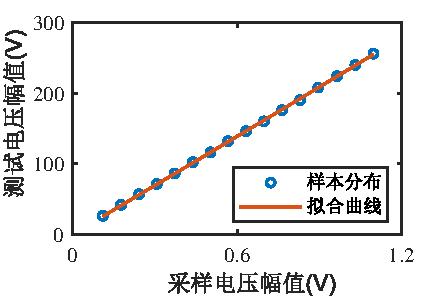
\includegraphics[scale=1]{MATLAB_plot_files/outputfit_vol.pdf}}%}
	\subfloat[电流采样数据拟合]{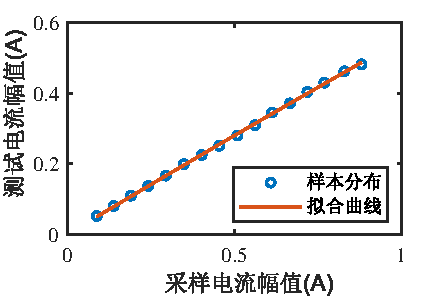
\includegraphics[scale=1]{MATLAB_plot_files/outputfit_cur.pdf}}%}
	\caption{最小二乘法数据拟合结果}\label{outputfit}
\end{figure}



\section{基于阻抗反馈的功率闭环控制系统设计}
被控对象分析，模型难以建立等因素
\subsection{ADRC控制算法}
工业控制中对于无模型控制对象通常采用PID控制算法，PID是一种基于误差反馈的控制律，通过当前误差、误差变化率以及误差积分的加权和来计算控制输入，其优势在于结构简单的同时易于理解和实现。然而，PID控制性能高度依赖于对象特性和参数整定结果，当被控对象存在较强非线性、时变特性或外部扰动时仅依靠误差反馈难以同时兼顾快速性、稳定性与鲁棒性。PID控制律如式(\ref{PID})所示：
\begin{equation}
	u(t) = K_p e(t) + K_i \int_{0}^{t} e(\tau) d\tau + K_d \frac{d e(t)}{d t}     \label{PID}
\end{equation}

为了克服PID控制器的局限性，韩京清在20世纪90年代提出自抗扰控制（Active Disturbance Rejection Control，ADRC）。ADRC是一类以总扰动估计与实时补偿为核心思想的控制方法，与经典控制方法依赖被控对象精确数学模型不同，ADRC并不要求完全确定对象内部全部动态机理，而是将模型不确定性、参数扰动、未建模动态以及外部扰动统一视为随时间变化的总扰动，并借助扩张状态观测器对其进行在线估计，最后在控制律中实现前馈补偿。由于其弱模型依赖与强扰动抑制的设计思想，ADRC在参数变化明显、外界扰动复杂与对象精确建模困难的控制场合中表现出较强的适用性。典型的ADRC结构主要由跟踪微分器（TD）、扩张状态观测器（ESO）以及非线性状态误差反馈控制律（NLSEF）三部分组成，分别承担参考信号平滑过渡、系统状态与总扰动估计、以及闭环控制量生成的功能。ADRC的经典控制结构如图\ref{ADRC}所示。
\begin{figure}[htbp]
	\centering
	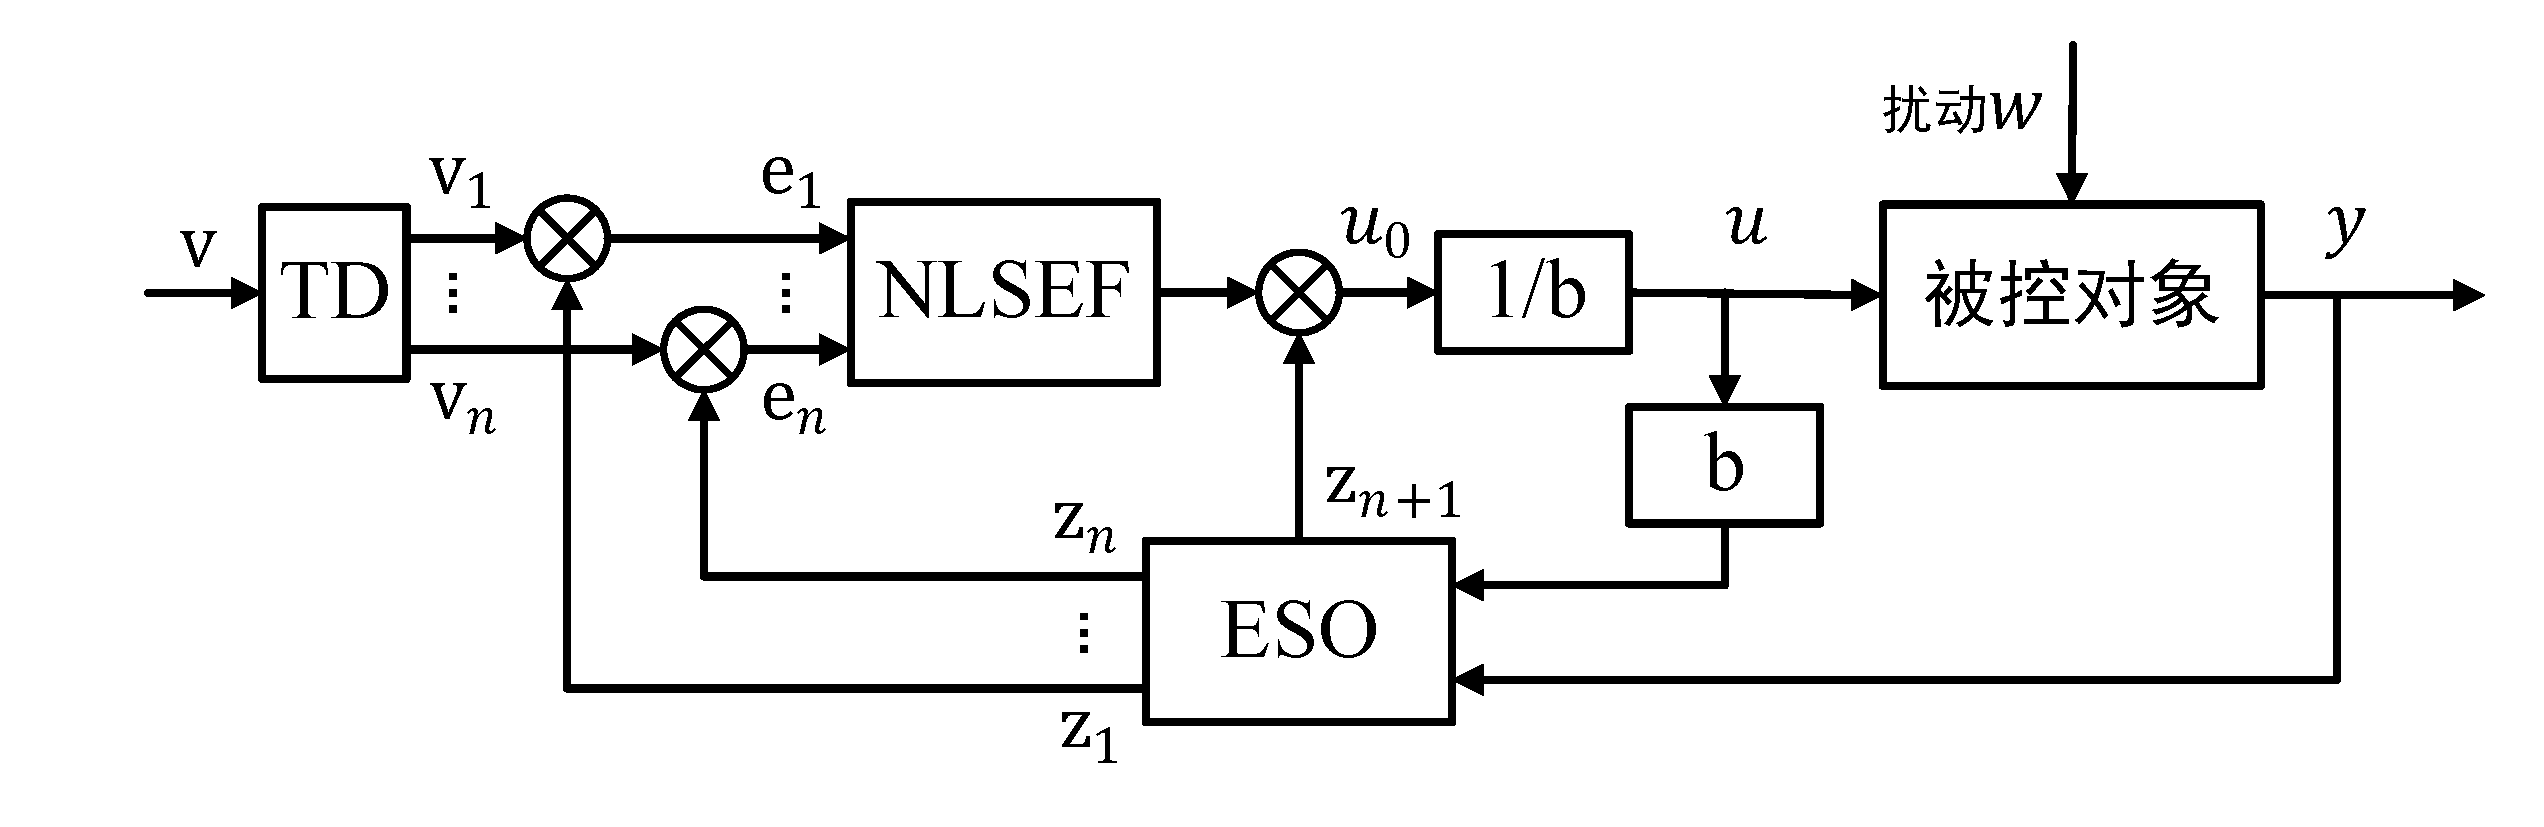
\includegraphics[scale=0.33]{Fig/ADRC.pdf}
	\caption{\label{ADRC}ADRC控制结构图}
\end{figure}

在工程实现中，ADRC通常包含较多耦合关系较强的非线性参数，整定过程极为依赖人工经验，同时在实际嵌入式系统中当采样频率有限、测量噪声明显时，过强的非线性观测与反馈机制可能引入抖振、噪声敏感或参数整定困难等问题。为此，高志强在ADRC的基础上提出了线性化实现方式，即线性自抗扰控制（LADRC）。LADRC在结构上与ADRC保持一致，但在具体实现上使用线性增益取代NLSEF与ESO的非线性函数，同时在多数应用场合中省略TD的复杂非线性结构，从而使得控制器参数数量显著减少，并可借助环路带宽调节的思想进行参数整定。对于一阶系统，设系统可表示为：
\begin{equation}
	\dot{y}=f ( y , t , w )+b u \label{ladrc:system}
\end{equation}
其中$y$为系统输出，$u$为控制输入，$f(y,t,w)$包含未知模型、参数不确定性以及外部扰动，$b$为控制增益增益。令$x_1=y$，$x_2=f(y,t,w)$，则系统扩张状态空间方程为：
\begin{equation}
	\begin{gathered}
		\begin{cases} {\dot{\mathbf{x}}=\mathbf{A} \mathbf{x}+\mathbf{B} u+\mathbf{E} \dot{f}} \\ {y=\mathbf{C} \mathbf{x}} \\ \end{cases} \\
		\renewcommand{\arraystretch}{0.85}       %控制间距
		\mathbf{A}=\left[ \begin{matrix} {0} & {1} \\ {0} & {0} \\ \end{matrix} \right], \quad \mathbf{B}=\left[ \begin{matrix} {b} \\ {0} \\ \end{matrix} \right],\quad \mathbf{E}=\left[ \begin{matrix} {0} \\ {1} \\ \end{matrix} \right], \quad \mathbf{C}=\left[ \begin{matrix} {1} & {0} \\ \end{matrix} \right]
	\end{gathered}\label{ladrc:state}
\end{equation}
式中$\mathbf{A}$为系统状态矩阵，$\mathbf{B}$为控制输入矩阵，$\mathbf{C}$为输出矩阵，$\mathbf{E}$为扰动输入矩阵，$f$可微并且$\dot{f}$有界。基于式(\ref{ladrc:system})，LADRC的线性扩张状态观测器为：
\begin{equation}
	\begin{gathered}
		\begin{cases} {\dot{\mathbf{z}}=\mathbf{A} \mathbf{z}+\mathbf{B} u+\mathbf{L} ( y-\hat{y} )} = (\mathbf{A}-\mathbf{L}\mathbf{C}) \mathbf{z}+\mathbf{L} y+\mathbf{B} u \\
			{\hat{y}=\mathbf{C} \mathbf{z}}                                                                                                                         \\
		\end{cases}
	\end{gathered}\label{ladrc:eso}
\end{equation}
其中$\mathbf{z}$为观测器状态向量，$\hat{y}$为观测器输出，$\mathbf{L}$为观测器增益矩阵，定义为$\mathbf{L}=[\beta_1, \beta_2]^T$。设$\mathbf{e}=\mathbf{x}-\mathbf{z}$为观测误差，观测误差系统的特征方程为$\lambda=\left| {\bf S I-( A-L C )} \right|=s^{2}+\beta_{1} s+\beta_{2}=\left( s+\omega_{o} \right)^{2} $，将观测器极点配置在$-\omega_{o}$处，则增益矩阵表示为$\mathbf{L}=[2\omega_o, \omega_o^2]^T$，$w_o$即为观测器带宽。LADRC的线性状态误差反馈控制律为：
\begin{equation}
	u = \frac{u_0-z_2} {b} = \frac{\alpha(r-z_1)-z_2} {b}       \label{ladrc:control}
\end{equation}
式中$u_o$为虚拟控制量，$\alpha$为控制器增益，$r$为参考输入。将式(\ref{ladrc:control})代入式(\ref{ladrc:system})，可得被控系统转换为积分环节，即$\dot{y}=(f ( y , t , w )-z_2)+u_0 = \alpha(r-z_1)$。设系统跟踪误差$e=r-y$，满足$\dot{e}=\dot{r}-\dot{y} = -\alpha e$，误差系统特征方程为$s+\alpha$，将控制器极点配置在$-\omega_c$处，则控制器增益表示为$\alpha=\omega_c$，$w_c$即为控制器带宽。

从上述算法推导可以看出，LADRC通过线性化的观测器与控制律设计，使得一阶系统中的总扰动在控制输入中被补偿，从而将系统简化为积分环节，通过虚拟控制器调节动态响应特性。同时，在带宽参数化的设计思想下，LADRC的参数调节过程将缩减为观测器带宽$w_o$、控制器带宽$w_c$以及控制增益$b$的调节，在调节过程中具有较为清晰的物理意义，且其参数通常满足$w_o \approx (3-5)w_c$，极大地降低了参数整定的难度。

由于LADRC最终需要在嵌入式系统中运行，需要将连续时间的算法公式转换为离散时间的实现形式。微控制器在实现数字控制时在离散采样时刻计算新的控制量，在相邻采样时刻之间保持控制值不变，对连续被控对象的作用呈现为分段常值信号，因此使用零阶保持器（ZOH）对连续时间LADRC进行离散化处理。设采样周期为$T_s$，各连续变量在每个采样区间$[kT_s, (k+1)T_s]$保持常值，系统扩张状态空间方程的离散化形式为：
\begin{equation}
	\begin{gathered}
		\begin{cases} {\mathbf{x} [ k+1 ]=\mathbf{\Phi} \mathbf{x} [ k ]+\mathbf{\Gamma} u [ k ]+\mathbf{\Gamma}_f} \overline{h} [k] \\ {y[k]=\mathbf{C} \mathbf{x}[k]} \\ \end{cases} \\
		\mathbf{\Phi}=e^{\mathbf{A} T_s} = \left[ \begin{matrix} {1} & {T_s} \\ {0} & {1} \\ \end{matrix} \right], \ \mathbf{\Gamma}=\int_{0}^{T_s} e^{\mathbf{A} \tau} \mathbf{B} d \tau = \left[ \begin{matrix} {b T_s} \\ {0} \\ \end{matrix} \right], \ \mathbf{\Gamma_f}=\int_{0}^{T_s} e^{\mathbf{A} \tau} \mathbf{E} d \tau = \left[ \begin{matrix} {\frac{T_s^2} {2}} \\ {T_s} \\ \end{matrix} \right]
	\end{gathered} \label{ladrc:discrete}
\end{equation}
式中，$\mathbf{\Phi}$为系统状态转移矩阵，$\mathbf{\Gamma}$为离散控制输入矩阵，$\mathbf{\Gamma_f}$为离散化的等效扰动矩阵，$\overline{h} [k]$为采样区间内扰动导数的等效平均值，若采样频率足够高且总扰动变化相对较慢，则此项对离散模型的影响可以视作一个小扰动项。扩张状态观测器的离散化形式为：
\begin{equation}
	\left\{
	\begin{aligned}
		z_1[k+1] & = z_1[k] + T_s z_2[k] + b T_s u[k] + l_1(y[k]-z_1[k]), \\    \label{ladrc:discrete_eso}
		z_2[k+1] & = z_2[k] + l_2(y[k]-z_1[k])
	\end{aligned}
	\right.
\end{equation}
式中，$l_1$和$l_2$为观测器增益参数。与连续时间的推导同理，误差系统的特征方程为$z^{2}+( l_{1}-2 ) z+\big( 1-l_{1}+T_{s} l_{2} \big)=0$，将观测器极点配置在$z_o=e^{-\omega_o T_s}$处，可解得增益参数为$l_{1}=2 {\left( {1-e^{-\omega_{o} T_{s}}} \right)}, l_{2}=\left( 1-e^{-\omega_{o} T_{s}} \right)^{2}/{T_{s}}$。当控制器采样频率远高于观测器带宽时，$e^{-\omega_{o} T_{s}} \approx 1-\omega_{o} T_{s}$，增益参数可近似表示为$l_1 \approx 2 \omega_o T_s$，$l_2 \approx \omega_o^2 T_s$。

离散控制律与连续时间形式相同，在采样时刻计算控制量输入，可表示为：
\begin{equation}
	u[k] = \frac{\alpha(r[k]-z_1[k])-z_2[k]} {b}       \label{ladrc:discrete_control}
\end{equation}
代入一阶系统方程，则系统输出更新可近似为$y [ k+1 ] \approx y [ k ]+T_{s} \alpha \bigl( r [ k ]-y [ k ] \bigr)$。定义系统离散形式下的跟踪误差为$e[k]=r[k]-y[k]$，误差系统特征方程为$z-( 1-\alpha T_{s} )=0$，将控制器极点配置在$z_c=e^{-\omega_c T_s}$处，则控制增益可表示为$\alpha = 1-e^{-\omega_{c} T_{s}}/T_{s} \approx \omega_c$。

式(\ref{ladrc:discrete_eso})与式(\ref{ladrc:discrete_control})即为一阶LADRC在零阶保持器条件下的离散实现形式。由此递推关系可以得到实际控制器中控制器实现的伪代码如列表\ref{ladrc_code}所示。
\begin{algorithm}
	\caption{一阶LADRC控制器实现伪代码}
	\label{ladrc_code}
	\begin{algorithmic}[1]
		\setlength{\baselineskip}{16pt} % 设置伪代码行间距
		\State \textbf{Input:} r, \ y, \ h, \ wo, \ wc, \ b
		\State \textbf{Initialization:}
		\State $\text{z1\_new} \gets 0$,\quad $\text{z1} \gets 0$
		\State $\text{z2\_new} \gets 0$,\quad $\text{z2} \gets 0$
		\State $\text{l1} \gets 2*wo*h$
		\State $\text{l2} \gets wo^2*h$
		\State \textbf{At each sampling instant:}
		\State $\text{e} \gets y-z1$
		\State$\text{z1\_new} \gets z1 + h*z2 + b*h*u + l1*e$
		\State$\text{z2\_new} \gets z2 + l2*e$

		\State$\text{z1} \gets \text{z1\_new}$,\quad $\text{z2} \gets \text{z2\_new}$
		\State$\text{u0} \gets wc*(r-z1)$
		\State$\text{u} \gets (u0-z2)/b$
		\State \textbf{Output:} u
	\end{algorithmic}
\end{algorithm}

\subsection{基于Simulink的仿真实验分析}
为验证LADRC控制策略在本文系统中的适用性与闭环控制性能，本文在Matlab/Simulink平台搭建闭环功率控制系统模型进行仿真实验分析。仿真模型由被控对象与离散 LADRC 控制器两部分构成，其中被控对象为第三章建立的高频能量发生电路，关键器件参数与实际电路保持一致，以尽可能真实地反映系统的动态特性；控制器则基于离散化的LADRC控制器实现，并按照数字控制系统的采样与更新方式嵌入闭环回路之中。通过对系统参考跟踪过程、扰动抑制能力及稳态调节效果的仿真分析，可为后续实验平台中控制器实现与参数整定提供依据。

Simulink作为一种面向多领域动态系统建模与仿真的集成环境，能够实现被控对象建模、控制器设计以及闭环响应分析的统一平台化开发。对于本文设计的高频电力电子系统，由于既包含开关器件的非线性动态行为，又涉及控制算法的离散实现，因此在仿真建模过程中采用分层建模方式：被控对象部分基于Simscape Electrical Specialized Power Systems模块中的功率电子库构建；控制器部分则基于Simulink基础模块库实现，通过增益、积分器、延时与离散环节等模块构建控制算法结构，并结合信号源与示波器等模块完成系统激励与响应观测。

\subsubsection{被控对象模型仿真}
在高频能量发生电路结构中，推挽逆变电路和LC谐振网络拓扑结构相对明确，可使用库中的基础元器件快速搭建。但对于由降压稳压芯片构成的可调直流源部分，仿真库中并未提供对应型号的器件模型，且其内部控制机制与补偿网络结构较为复杂，难以通过简单的分立元件等效实现；若直接采用理想直流电压源进行替代则会忽略该部分电路的动态调节特性。因此，本文以典型Buck变换器进行等效替代，通过合理设计电感、电容及控制参数，使其尽可能逼近可调直流源的调节行为，从而提高控制器设计与仿真验证的工程参考价值。Buck电路的设计参数如表\ref{buck_param}所示。
\begin{table}[htbp]
	\caption{\label{buck_param}Buck电路设计参数}
	\centering
	\small
	\setlength{\tabcolsep}{20pt}
	\begin{tabular}{c c c c }
		\hline
		参数      & 数值        & 参数      & 数值        \\
		\hline
		输入电压    & 50V       & 输出电压    & 20V       \\
		输出功率    & 100W      & 开关频率    & 100KHz    \\
		电感电流纹波率 & 20\%      & 电容电压纹波率 & 2\%       \\
		电感值     & 80$\mu$ H & 电容值     & 47$\mu$ F \\
		\hline
	\end{tabular}
\end{table}

Buck电路本质上是包含储能环节的二阶系统，其输出电压不仅受输入电压的影响，同时还与负载变化及开关占空比密切相关。在开环控制条件下，输出电压在出现扰动时难以稳定在设定参考值，因此必须引入闭环控制策略。针对Buck电路的动态特性及控制需求，本文采用电压外环与电感电流内环构成的串级双闭环控制结构，其中外环以输出电压为控制量，通过电压误差生成电流给定；内环则以电感电流为调节对象，通过快速调节开关占空比使实际电感电流能够快速跟踪给定值，从而提高系统对输入变化和负载扰动的响应速度，内外环控制器均采用PID控制器。仿真电路结构如图\ref{buck_control}所示。
\begin{figure}[htbp]
	\centering
	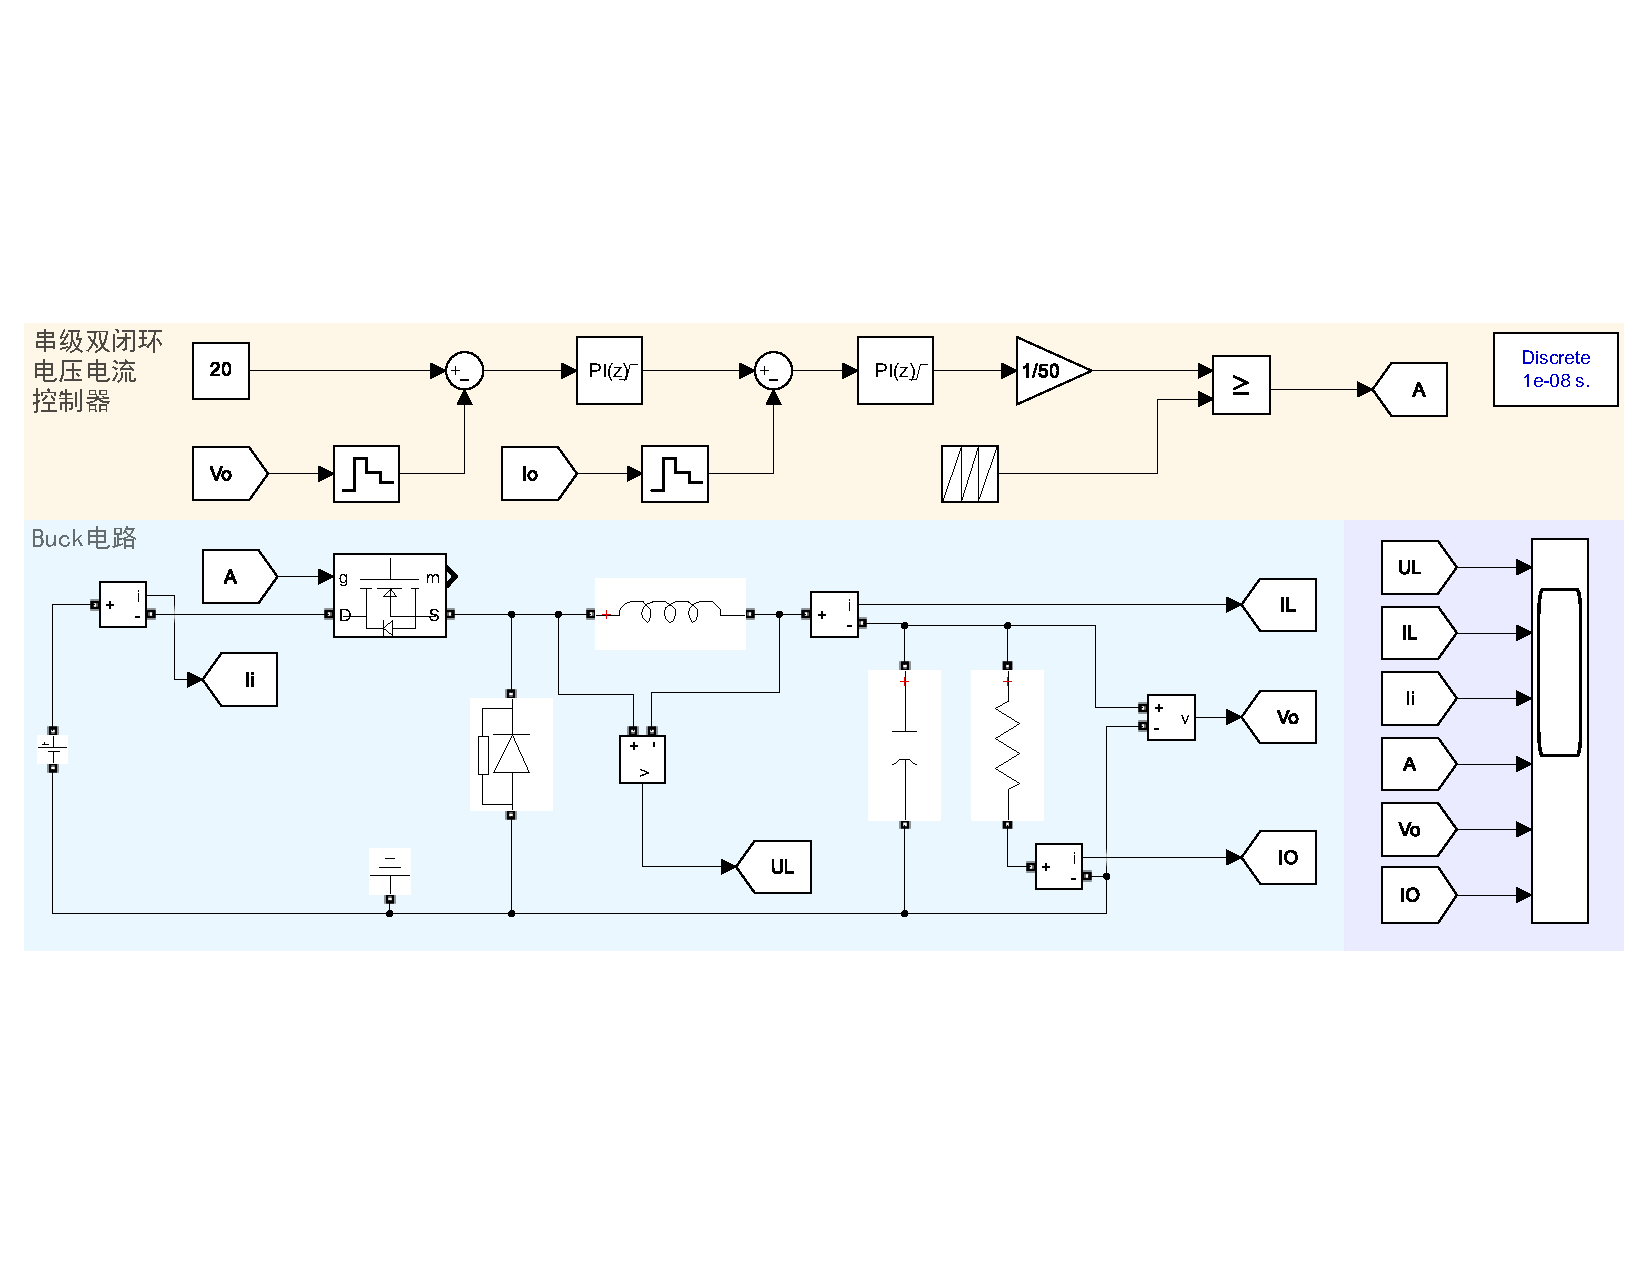
\includegraphics[scale=0.58]{MATLAB_plot_files/buck_control_fig.pdf}
	\caption{\label{buck_control}Buck电路及其闭环控制器仿真结构图}
\end{figure}

在Simulink仿真中，系统整体采用离散时间定步长求解方式，固定步长设置为10ns；控制器结构中离散PID控制器和零阶保持器采样时间均与开关周期一致，设为10us。在上述仿真条件下，Buck电路的时域及频域响应仿真结果如图\ref{buck_result}所示。
\begin{figure}[htbp]
	\centering
	\subfloat[开环电压阶跃响应]{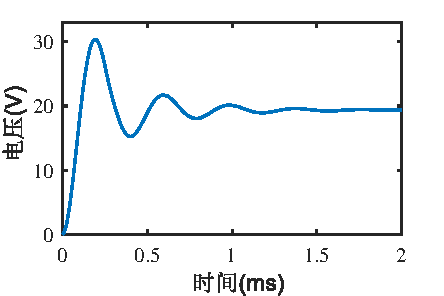
\includegraphics[scale=1]{MATLAB_plot_files/buck_open_t.pdf}
		\label{buck_control:a}}
	\subfloat[闭环电压阶跃响应]{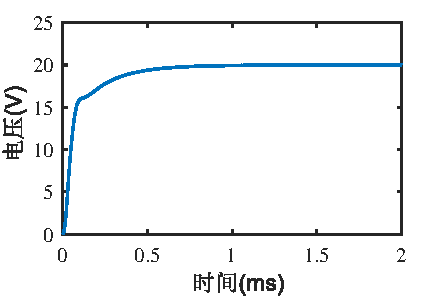
\includegraphics[scale=1]{MATLAB_plot_files/buck_close_t.pdf}
		\label{buck_control:b}} \\
	\subfloat[开环伯德图]{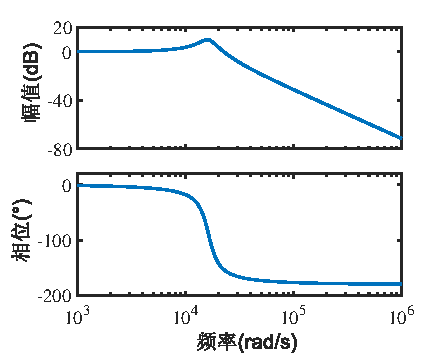
\includegraphics[scale=1]{MATLAB_plot_files/buck_open_f.pdf}
		\label{buck_control:c}}%}
	\subfloat[控制器校正后伯德图]{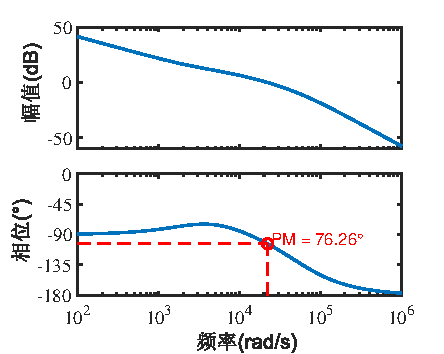
\includegraphics[scale=1]{MATLAB_plot_files/buck_close_f.pdf}
		\label{buck_control:d}}
	\caption{Buck电路时域及频域响应对比}  \label{buck_result}
\end{figure}

如图\ref{buck_control:a}与\ref{buck_control:b}所示，在占空比为0.4的阶跃输入下，开环Buck电路输出电压在调节过程中存在明显振荡，调节时间较长，且与目标值20V之间存在稳态误差；引入电压电流双闭环控制结构后，系统的动态性能得到显著改善，闭环系统在20V阶跃输入下实现无超调的快速响应，稳态误差得到有效消除。从频域特性来看，如图\ref{buck_control:c}与\ref{buck_control:d}所示，控制器校正后系统在低频段具有更高的开环增益，在中频段以约-20dB/dec的斜率穿越0dB增益线，穿越频率约为22.2KHz，具有充足的相位裕度和较好的闭环带宽。此外幅频响应中原有的谐振峰值消除，在时域上表现为系统的超调量与调节时间减小。上述仿真结果表明，双闭环控制策略能够显著优化Buck电路的动态与稳态性能，从而可以较好地模拟实际可调降压稳压电路的动态特性。
\begin{figure}[htbp]
	\centering
	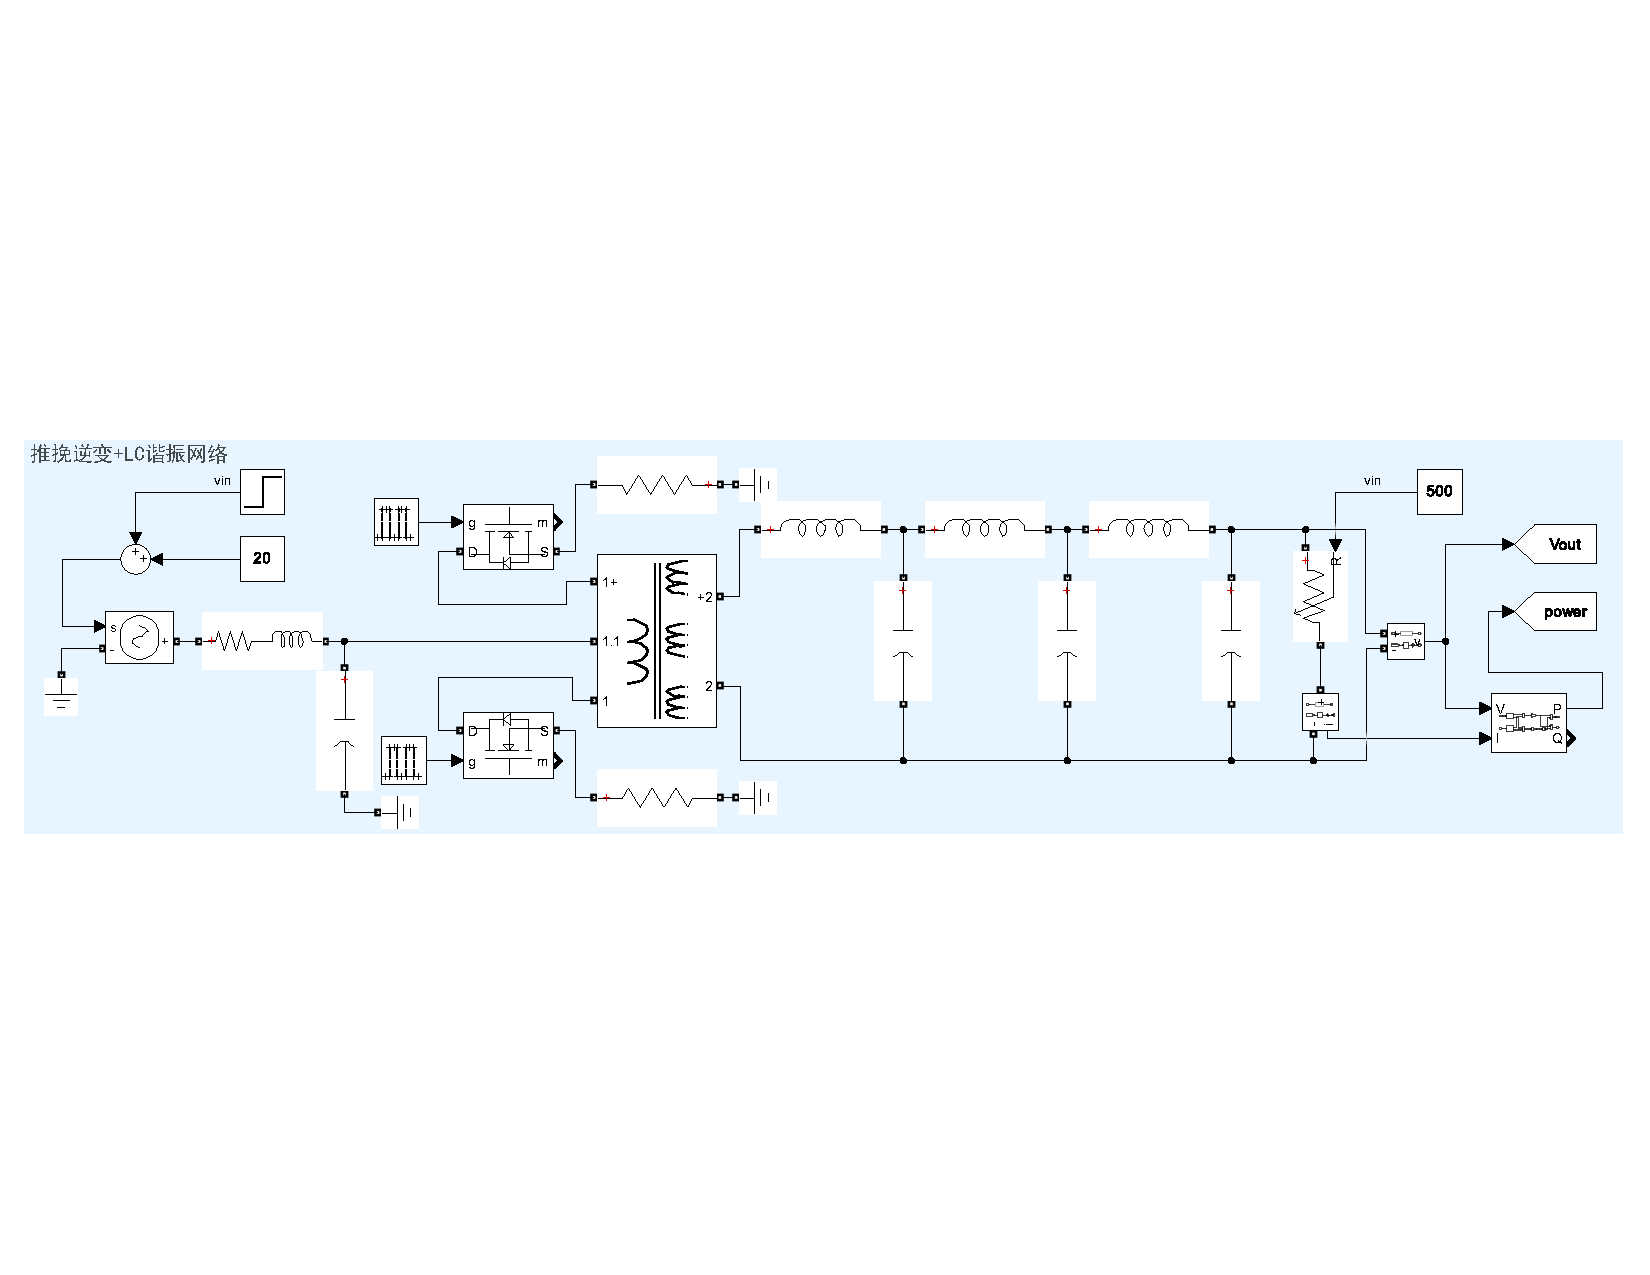
\includegraphics[scale=0.59]{MATLAB_plot_files/pushpull_lc_fig.pdf}
	\caption{\label{pushpull_lc}高频逆变及选频滤波电路仿真结构图}
\end{figure}

高频逆变及选频滤波电路的仿真结构如图\ref{pushpull_lc}所示。该仿真系统中使用理想电压源为变压器中心抽头提供输入电压，以避免前级电源对逆变过程动态分析干扰；输出侧负载使用可变电阻模块，以便在后续仿真实验中灵活引入负载扰动；负载端配置电压、电流测量模块对输出信号进行采样，并结合功率模块提取350KHz基频下的输出功率。在额定负载、输入电压施加20V阶跃变化的条件下，电路输出的时域响应如图\ref{pushpull_lc_result}所示。
\begin{figure}[htbp]
	\centering
	\subfloat[开环电压阶跃响应]{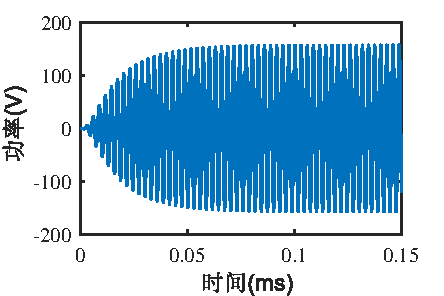
\includegraphics[scale=1]{MATLAB_plot_files/pushpuull_lc_v.pdf}}%}
	\subfloat[开环功率阶跃响应]{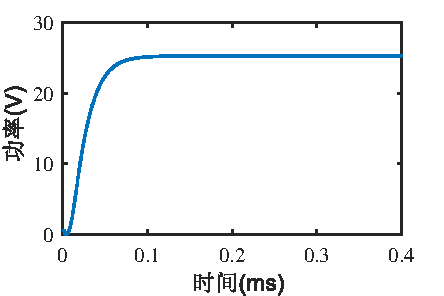
\includegraphics[scale=1]{MATLAB_plot_files/pushpuull_lc_p.pdf}}%}
	\caption{高频逆变及选频滤波电路时域响应} \label{pushpull_lc_result}
\end{figure}

由仿真结果可以看出，所搭建电模型在直流电压输入下能够稳定输出频率为350KHz正弦交流电压波形，且输出电压及功率在电压阶跃输入下迅速完成过渡过程并稳定在目标值附近，调节时间约为0.1ms。由此可见在能量发生电路仿真模型中，前级Buck电路与后级高频逆变及选频滤波电路均能够较好地模拟实际系统的稳态输出特性，且均有1e-4时间级的较快动态响应过程。
\subsubsection{闭环控制仿真}
在上述被控对象电路模型的基础上，本文将离散化的LADRC控制器嵌入系统闭环回路中进行仿真验证。在所构建的闭环功率控制系统中，LADRC作为外层功率调节器，以系统输出功率为控制对象，输出作为前级Buck电路双闭环控制结构中的电压参考输入，从而实现对系统输出功率的简介调控。功率闭环控制系统结构如图\ref{control_struct}所示。
\begin{figure}[htbp]
	\centering
	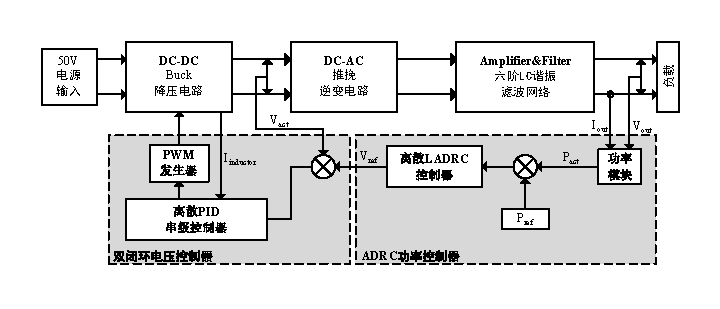
\includegraphics[scale=1.3]{Fig/control_struct.pdf}
	\caption{\label{control_struct}功率闭环控制系统结构图}
\end{figure}

LADRC控制器的离散化实现基于前向欧拉法的离散时间积分器与零阶保持器实现。在仿真中功率控制器的采样周期设为50us，由于被控量输出功率与控制输入电压之间存在确定的非线性映射关系，因此在LADRC控制器中引入前馈补偿结构，从而在参考值变化或外部扰动时提供先验调节量。闭环功率控制系统的仿真结构如图\ref{hf_system}所示。
\begin{figure}[htbp]
	\centering
	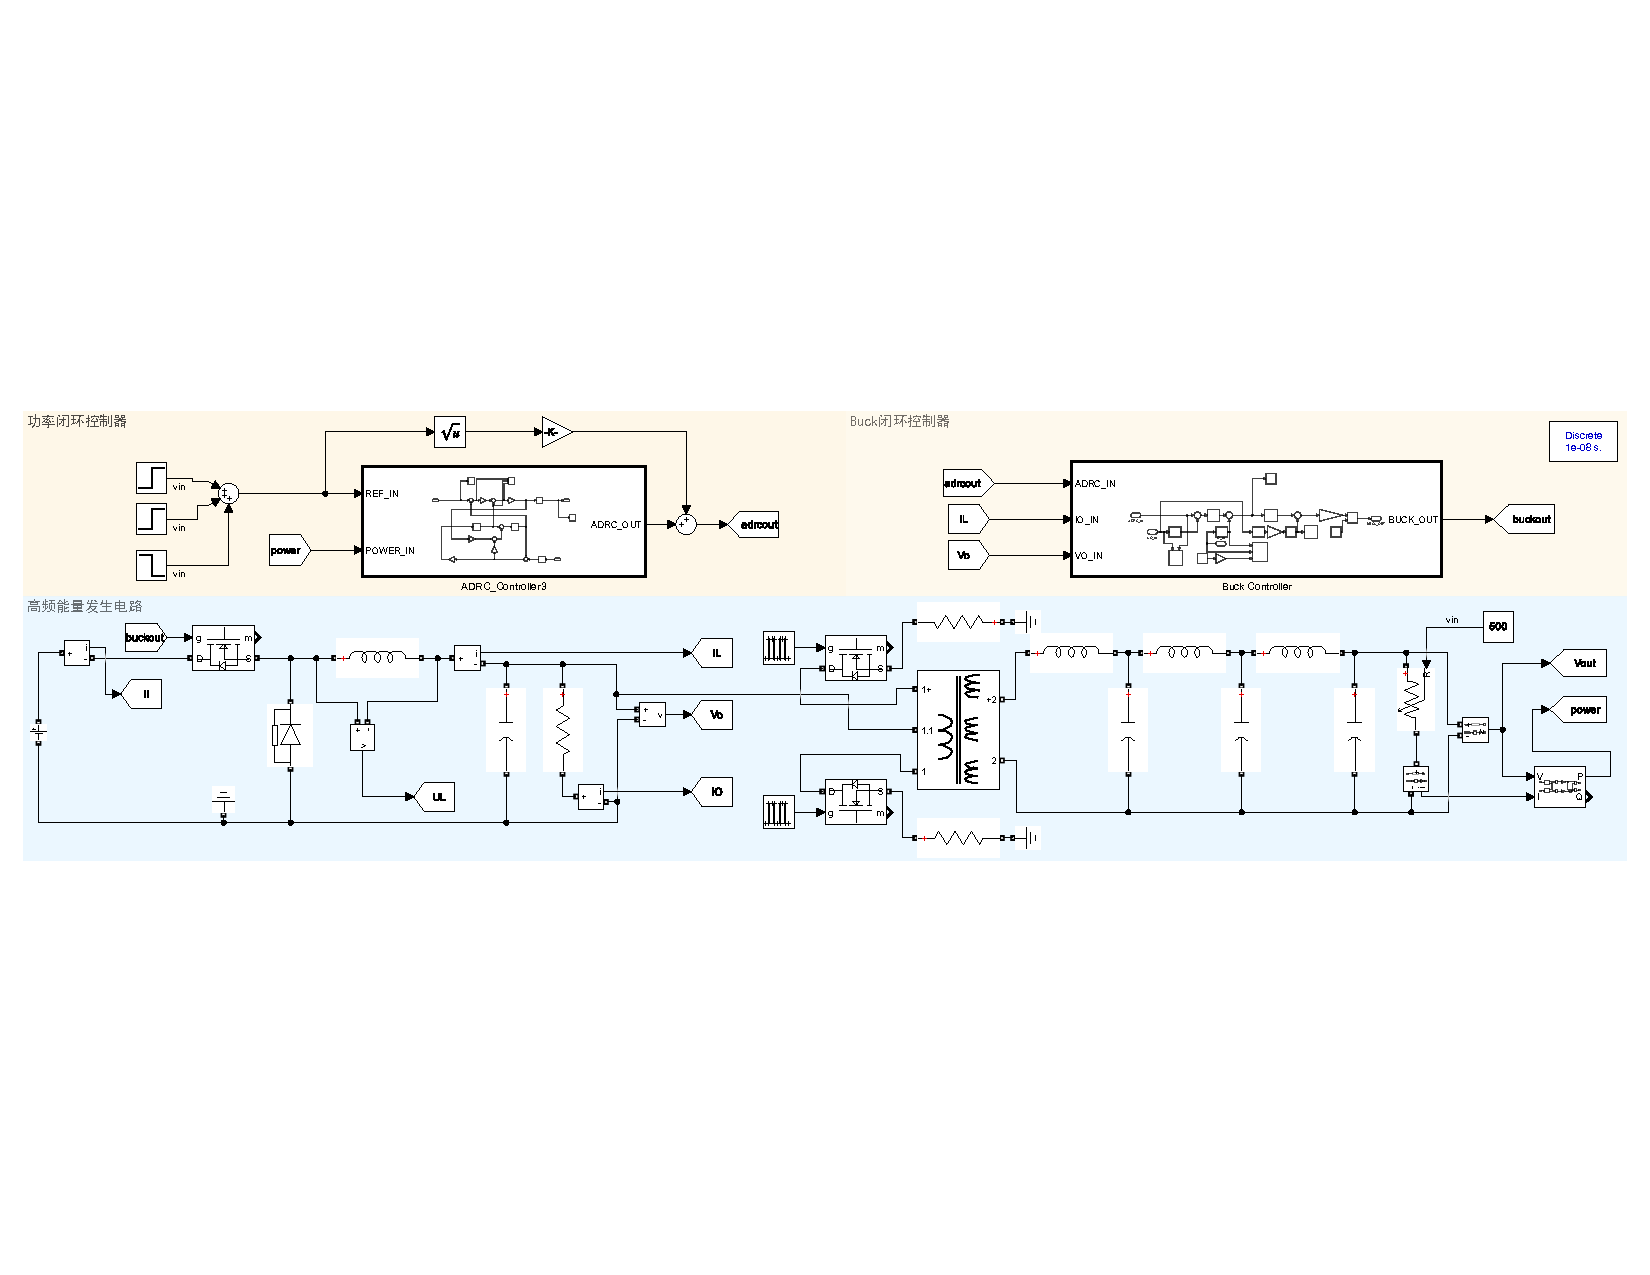
\includegraphics[scale=0.57]{MATLAB_plot_files/hf_system_fig.pdf}
	\caption{\label{hf_system}闭环功率控制系统仿真结构图}
\end{figure}

在20W稳态输出条件下，分别于20ms与40ms时刻施加20W功率阶跃输入，仿真结果如图\ref{hf_p}所示。由仿真结果可以看出，系统在一阶LADRC控制器的调节下能够迅速跟踪到新的功率设定值。在相同的控制器参数配置下引入前馈补偿，系统响应速度进一步提升，调节时间缩短约3ms，且在过渡过程中没有引入明显的超调现象。同时需要注意的是，引入前馈补偿后动态过渡初期出现了一定幅度的尖峰现象，这主要是由于前馈通道在阶跃输入时产生瞬时控制量突变导致系统短时激励增强。从整体响应过程来看，该尖峰并未引入明显的超调，也未对系统稳定性造成不利影响。
\begin{figure}[htbp]
	\centering
	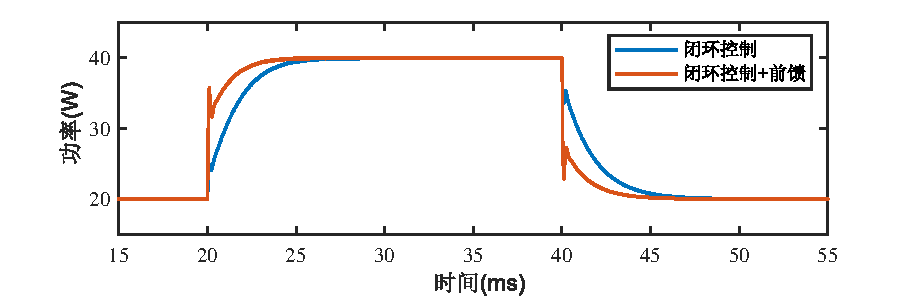
\includegraphics[scale=1]{MATLAB_plot_files/hf_p.pdf}
	\caption{\label{hf_p}闭环功率阶跃响应}
\end{figure}

为验证LADRC功率闭环控制器在负载扰动条件下的性能，本文模拟高频电外科发生器工作过程中负载变化，在可变电阻模块中引入负载扰动信号，即在500Ω稳定负载条件下于20ms处引入斜率为5000的斜坡信号，并于30ms处引入均值为200，方差为600的正态分布随机信号，负载扰动信号如图\ref{hf_load}所示。在此负载扰动信号的作用下，系统的功率响应如图\ref{hf_p_disturbance}所示。

\begin{figure}[htbp]
	\centering
	\begin{minipage}[c]{0.5\textwidth}
		\centering
		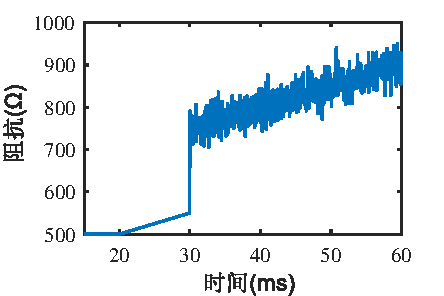
\includegraphics[scale=1]{MATLAB_plot_files/hf_load.pdf} %1:1导入
	\end{minipage}%
	\begin{minipage}[c]{0.5\textwidth}
		\centering
		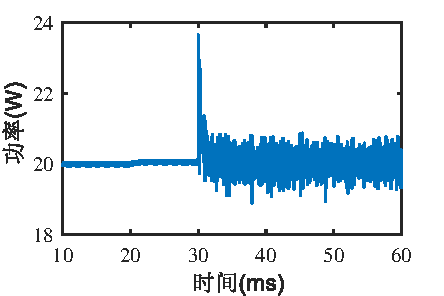
\includegraphics[scale=1]{MATLAB_plot_files/hf_p_disturbance.pdf}
	\end{minipage}\\[1pt]
	\begin{minipage}[t]{0.5\textwidth} % 以下为新添加页面划分，[t]表示行顶部对齐
		\caption{\label{hf_load}负载扰动信号}
	\end{minipage}%
	\begin{minipage}[t]{0.5\textwidth}
		\caption{\label{hf_p_disturbance}负载扰动下的闭环功率响应}
	\end{minipage}%
\end{figure}
由仿真结果可知，在设定功率为20W的条件下，负载引入斜坡扰动后在控制器调节的作用下，输出功率时钟稳定在参考值附近，未出现明显的持续性偏移，表明系统对缓变扰动具有良好的抑制能力；当进一步叠加符合正态分布的随机扰动后，由于扰动引入瞬间等效为负载阻抗的突变，系统输出功率出现瞬态响应，产生约24 W的瞬时尖峰，随后在控制器快速调节作用下功率在约1.5ms内迅速收敛至稳态值附近，并且在后续的随机扰动与斜坡扰动的共同作用下，维持在设定值 ±0.8 W 的波动范围内，体现出较强的抗扰动能力与稳态保持性能。此外在仿真过程中可以观察到，当扩张状态观测器带宽设置较大时，控制器对于扰动的观测与补偿能力增强，从而使输出功率的稳态偏差进一步减小，与LADRC的设计思想相符。

对与恒电压控制和恒电流控制场景，本文同样采用一阶LADRC控制器进行仿真验证，其中电压控制器以负载两端电压有效值为被控量，输入为150V电压阶跃；电流控制器以负载电流有效值为被控量，输入为0.3A电流阶跃。同时两种控制模式下均在20ms处施加与功率控制相同的负载扰动信号，仿真结果如图\ref{hf_vc_cc}所示。
\begin{figure}[htbp]
	\centering
	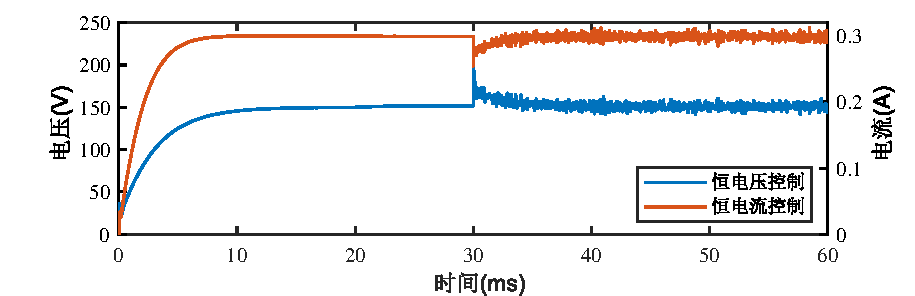
\includegraphics[scale=1]{MATLAB_plot_files/hf_vc_cc.pdf}
	\caption{\label{hf_vc_cc}恒电压与恒电流控制仿真结果}
\end{figure}
在阶跃输入作用下，电压电流输出均能快速上升并稳定在参考值附近。在引入负载扰动信号后，输出电压和电流仅在扰动引入瞬间出现瞬态尖峰，随后在控制器的调节作用下迅速收敛到稳态值附近，体现出较快的动态响应能力。引入负载扰动信号后，输出信号仅在扰动作用瞬间出现短时尖峰响应，随后迅速收敛到稳态值附近，在后续扰动的持续作用下维持在设定值±8V和±0.02A的波动范围内，表明系统具有良好的抗扰动能力与稳态保持性能。

综合恒功率、恒电压与恒电流三种控制模式下的仿真结果可以看出，不同控制目标与负载扰动条件下同时实现较快的动态响应与较高的稳态精度，具有较强的鲁棒性与适应性，能够满足高频电外科发生器在多工作模式下的控制需求。

\section{双核处理器协同程序设计}
由前文3.4.2节控制单元架构设计可知，本文所设计系统采用双核处理器架构，并通过定时信号实现周期性的同步运行。在此硬件架构的基础之上，双核软件需完成的功能根据系统整体的功能需求可分为输出信号同步采样、频域分析及信号处理、闭环控制及驱动以及人机交互数据传输四个模块。为将上述功能模块高效分配到双核处理器的控制周期内，本文首先根据各模块的处理器计算时间进行任务规划与功能划分。

在 STM32 微控制器中，DWT是ARM Cortex-M内核提供的片上调试与跟踪单元，其内部周期计数器CYCCNT能够以处理器内核时钟为基准进行连续计数，从而可以以亚微秒量级高精度测量程序运行时间，适用于实时控制系统的关键代码执行开销分析。本文通过在各功能模块的关键代码段前后插入DWT计数器的读取指令，可以获取每个模块的实际执行周期数，并结合处理器时钟频率计算出对应的执行时间。系统主要程序模块DWT计算耗时分析结果如表\ref{dwt_time}所示。
\begin{table}[htbp]
	\caption{\label{dwt_time}核心代码模块执行耗时}
	\centering
	\small
	\setlength{\tabcolsep}{20pt}
	\begin{tabular}{c c c c }
		\hline
		程序模块名称       & 耗时（ms） & 程序模块名称  & 耗时（ms） \\
		\hline
		信号加窗处理       & 0.5115 & 同步信号采样  & 0.5068 \\
		Goertzel频域分析 & 0.4693 & 闭环控制及驱动 & 0.0543 \\
		输出信号滤波       & 0.0129 & 双机数据传输  & 0.0029 \\
		\hline
	\end{tabular}
\end{table}

由此可见，耗时较长的任务主要集中在同步信号采样、信号加窗处理以及Goertzel频域分析三个模块，分别占用约0.5ms的处理时间。上述三个程序模块从功能划分的角度看，均属于对于高频输出信号的采样和处理，因此由隔离区的微控制器负责执行和处理，而非隔离区的微控制器由于需要提供能量发生电路驱动并与人机交互板连接，因此自然而然负责执行闭环控制驱动以及用于人机交互的数据传输。

然而，耗时较长的程序模块属于信号处理与分析流程，若依次执行则隔离区微控制器执行周期在保留裕度的情况下至少要设置为3ms，在双核同步运行的设计中将导致非隔离区的微控制器计算资源利用率较低。为此，本文使用DMA数据传输机制实现信号采样与频域分析的并行化处理。DMA是微控制器内提供的直接存储器访问外设，核心作用是在不占用CPU资源的情况下实现外设与内存之间的数据传输。本文通过配置DMA控制器，使其在ADC同步连续采样1022点时将采样数据直接传输到预设的内存区，与此同时触发CPU执行Goertzel频域分析算法，从而在0.5ms的采样时间内同时完成两个功能模块的处理，同时保证采样结果与加窗过程不会产生数据冲突。在此设计下，双机同步的控制周期可缩短至1.5ms，非隔离区微控制器的计算资源得到更高效的利用。基于程序运行耗时测量和DMA机制的程序任务规划及时序如图\ref{task_plan}所示。
\begin{figure}[htbp]
	\centering
	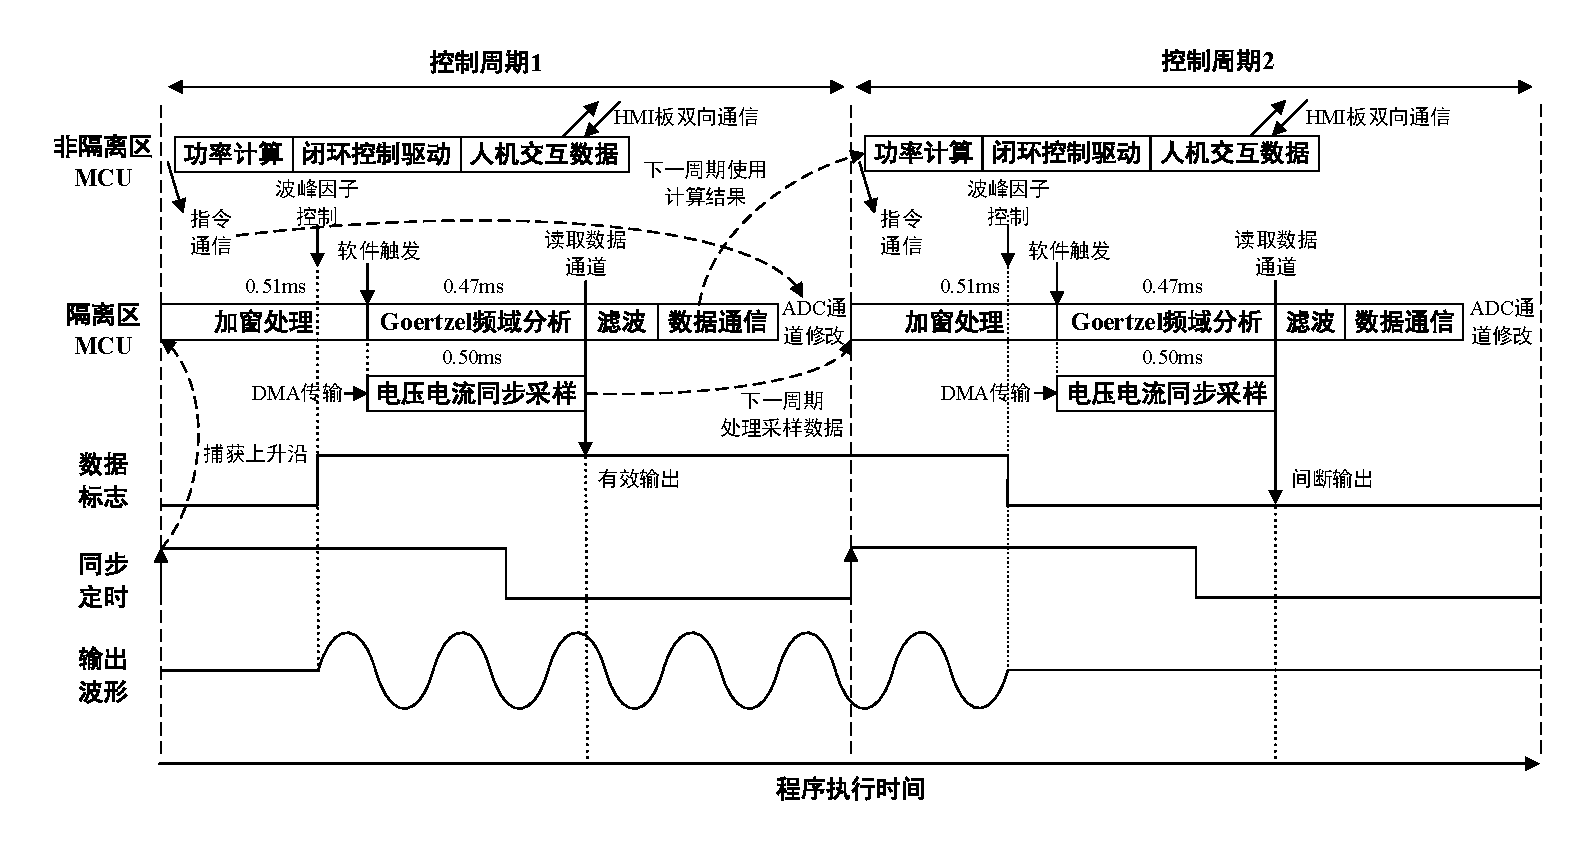
\includegraphics[scale=0.63]{Fig/timing.pdf}
	\caption{\label{task_plan}程序任务规划及时序}
\end{figure}

图中未标识时间的程序模块均耗时极短，其框图长度不代表实际执行时间。时序图中提供了两个控制周期内双核处理器的程序执行情况，也绘制出了控制单元架构中交互数据以及输出波形。可见在双处理器同步定时下，两个区域微控制器中所有任务执行始末时刻均可确定，从而可以控制特定程序的执行位置，例如非隔离区MCU在控制周期起始发送ADC通道变更指令，为避免在采样过程中修改ADC工作方式导致的问题，隔离区MCU接收指令后在当前控制周期所有任务执行完成后再进行ADC通道切换，从而保证了系统的稳定性与可靠性。

此外从时序图中可以看出，在引入DMA机制后，隔离区MCU的频域分析和同步采样的处理时间重叠，由此本周期内的采样数据在下一个控制周期内才能进行数据处理与频域分析，同时由于向非隔离区MCU发送计算结果的数据通信部分位于控制周期末尾，因此本周期内的频域分析结果只能在下一个控制周期内用于闭环控制和驱动。从而形成了类似于流水线的处理流程，如图\ref{pipeline}所示。此种方式虽然引入一定的数据从采样到控制的延时，但是通过缩小控制周期的方式提高了采样和控制的频率，整体上对系统性能的提升具有积极作用。
\begin{figure}[htbp]
	\centering
	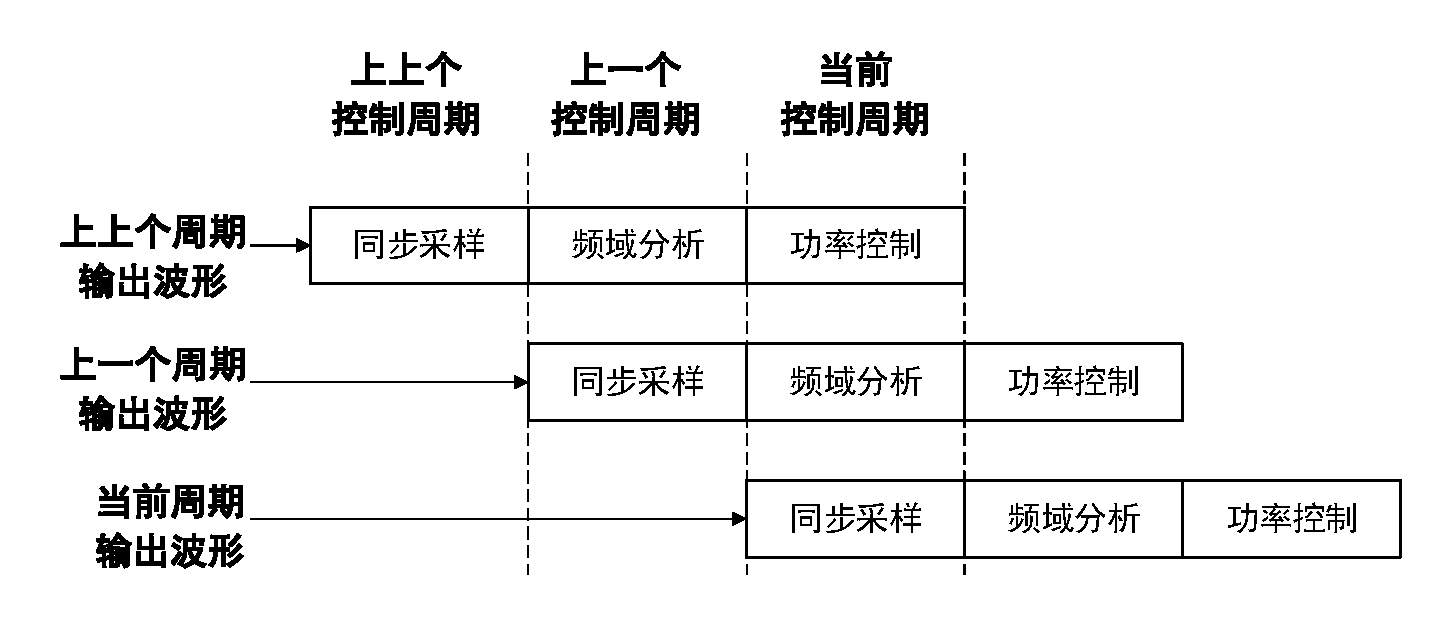
\includegraphics[scale=0.55]{Fig/pipeline.pdf}
	\caption{\label{pipeline}流水线式信号处理流程}
\end{figure}

双处理器架构高度依赖通过隔离模块的串口通信来完成数据和指令的交换，其中非隔离区MCU主要发送频域分析得到的幅值和相位差信息，隔离区MCU主要发送工作模式以控制ADC采样配置。为加快通信时间并减少处理器的干预，本文在通信过程中使用DMA传输串口数据，通过串口空闲中断完成数据接收，并设计了数据帧结构以实现数据的有效解析与处理。通信指令帧设计如图\ref{comm_frame}所示，帧结构由帧头、数据位、校验和和帧尾组成，在数据解析过程中只有当帧头和帧尾正确匹配，且所有数据累加运算与帧中的校验和一致时，才会认为数据有效并执行和处理，从而防止通信错误导致的系统工作异常问题。
\begin{figure}[htbp]
	\centering
	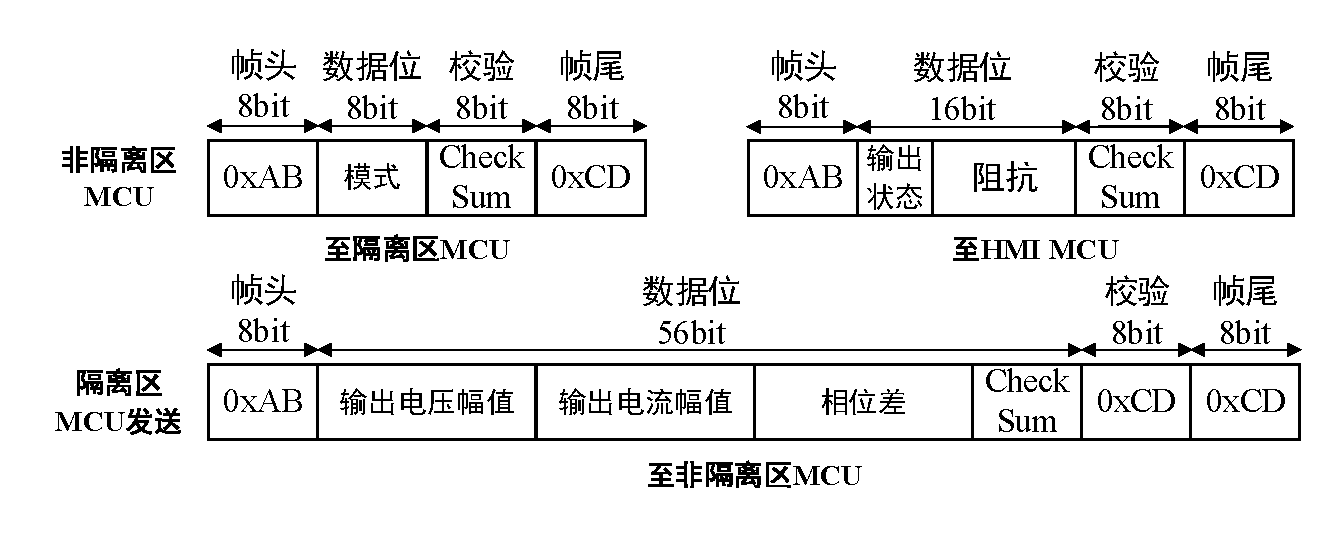
\includegraphics[scale=0.6]{Fig/comm_frame.pdf}
	\caption{\label{comm_frame}双机通信指令帧设计}
\end{figure}

本系统中的两个核心程序流程输出功率控制与有功功率控制均围绕上述所设计双核处理器软件架构和任务规划进行展开，具体程序流程在下面的小节中进行详细介绍。

\subsection{输出模式控制}
高频电外科发生器系统不同输出模式下的输出波形不同，主要通过波峰因子来衡量输出波形的特征。波峰因子定义为系统输出电压峰值与其均方根值的比值，能够反映输出波形的尖锐程度和能量集中程度。波峰因子的数学表达式为：
\begin{equation}
	CF = \frac{V_{peak}}{V_{rms}} = \frac{\max |v(t)|}{\sqrt{\frac{1}{T} \int_{0}^{T} v^2(t) dt}}
\end{equation}
由定义式可以看出，若系统可输出的最大峰值电压一定，有效输出时间与间断时间的比例越小，则有效值越低，从而具有更大的波峰因子。设交流正弦波形的有效输出时间占总周期的比例为$\alpha$，考虑到满占空比的正弦波波峰因子为$\sqrt{2}$，则其波峰因子可以表示为$CF = \sqrt{2\alpha}$。常见高频电外科发生器的输出模式及波峰因子参考值如表\ref{esu_cf}所示。
\begin{table}[htbp]
	\caption{\label{esu_cf}常见高频电外科发生器输出模式及波峰因子参考值}
	\centering
	\small
	\setlength{\tabcolsep}{5pt}
	\begin{tabular}{c c c c}
		\hline
		输出模式                     & 波峰因子参考值 & 输出模式              & 波峰因子参考值 \\
		\hline
		纯切（Pure Cut）             & 1.6     & 软凝（Soft Coag）     & 1.6     \\
		混切（Blend / Enhanced Cut） & 2.5     & 强凝（Forced Coag）   & 3.0     \\
		点凝（Pin Point Coag）       & 2.6     & 喷凝（Spray Coag）    & 8.5     \\
		电灼凝（Fulguration）         & 4.0     & 双极凝（Bipolar Coag） & 1.6     \\
		\hline
	\end{tabular}
\end{table}

本文通过控制系统输出间断时间不同的正弦波形来实现不同输出模式的控制，由于高频波形最初由推挽逆变器输出，因此可控制逆变电路中MOSFET的驱动波形的间断输出时间。在实验中发现，使用常规方式中断定时器的输出比较通道不能实现两路驱动PWM波形的同步关断，从而可能导致电源短路问题。为此，本文使用STM32高级定时器刹车机制来实现两路PWM波形的同步关断。具体而言，在需要产生间断时间的时刻通过软件触发定时器刹车事件，两通道驱动波形强制设置为空闲状态，并在间断时间结束后置位MOE控制位恢复PWM输出。

从输出功率的计算方式来看，若输出波形的有效输出占空比为$\alpha$，则此间断输出状态下的实际输出功率为$P_{active}/\alpha$，其中$P_{active}$为系统在有效输出持续时间内计算的功率。由此可见，系统仅需在有效输出时间内采样并计算输出功率，即可结合当前模式下的占空比$\alpha$计算出实际输出功率。为了辅助非隔离区MCU对当前输出状态的判断，在隔离通信模块中的一个数据通道设置为数据标志位，如图\ref{task_plan}所示。当系统需要控制产生一定波峰因子的输出波形时，非隔离区MCU通过计数器控制有效输出或间断时间的控制周期数并产生或中断驱动PWM波形，同时根据输出状态拉高或拉低数据标志位，非隔离区在执行频域分析时可通过数据标志位判断输出状态，若上一周期的数据标志位为高，则当前周期执行加窗和频域分析的数据为有效输出的采样数据，其幅值和相位差分析结果保留并用于功率计算；若为低则为间断输出的采样数据，将计算结果丢弃以避免在滤波过程中对功率计算造成的影响。

双核处理器同步架构下的输出模式控制程序流程图如图\ref{cf_control}所示。
\begin{figure}[htbp]
	\centering
	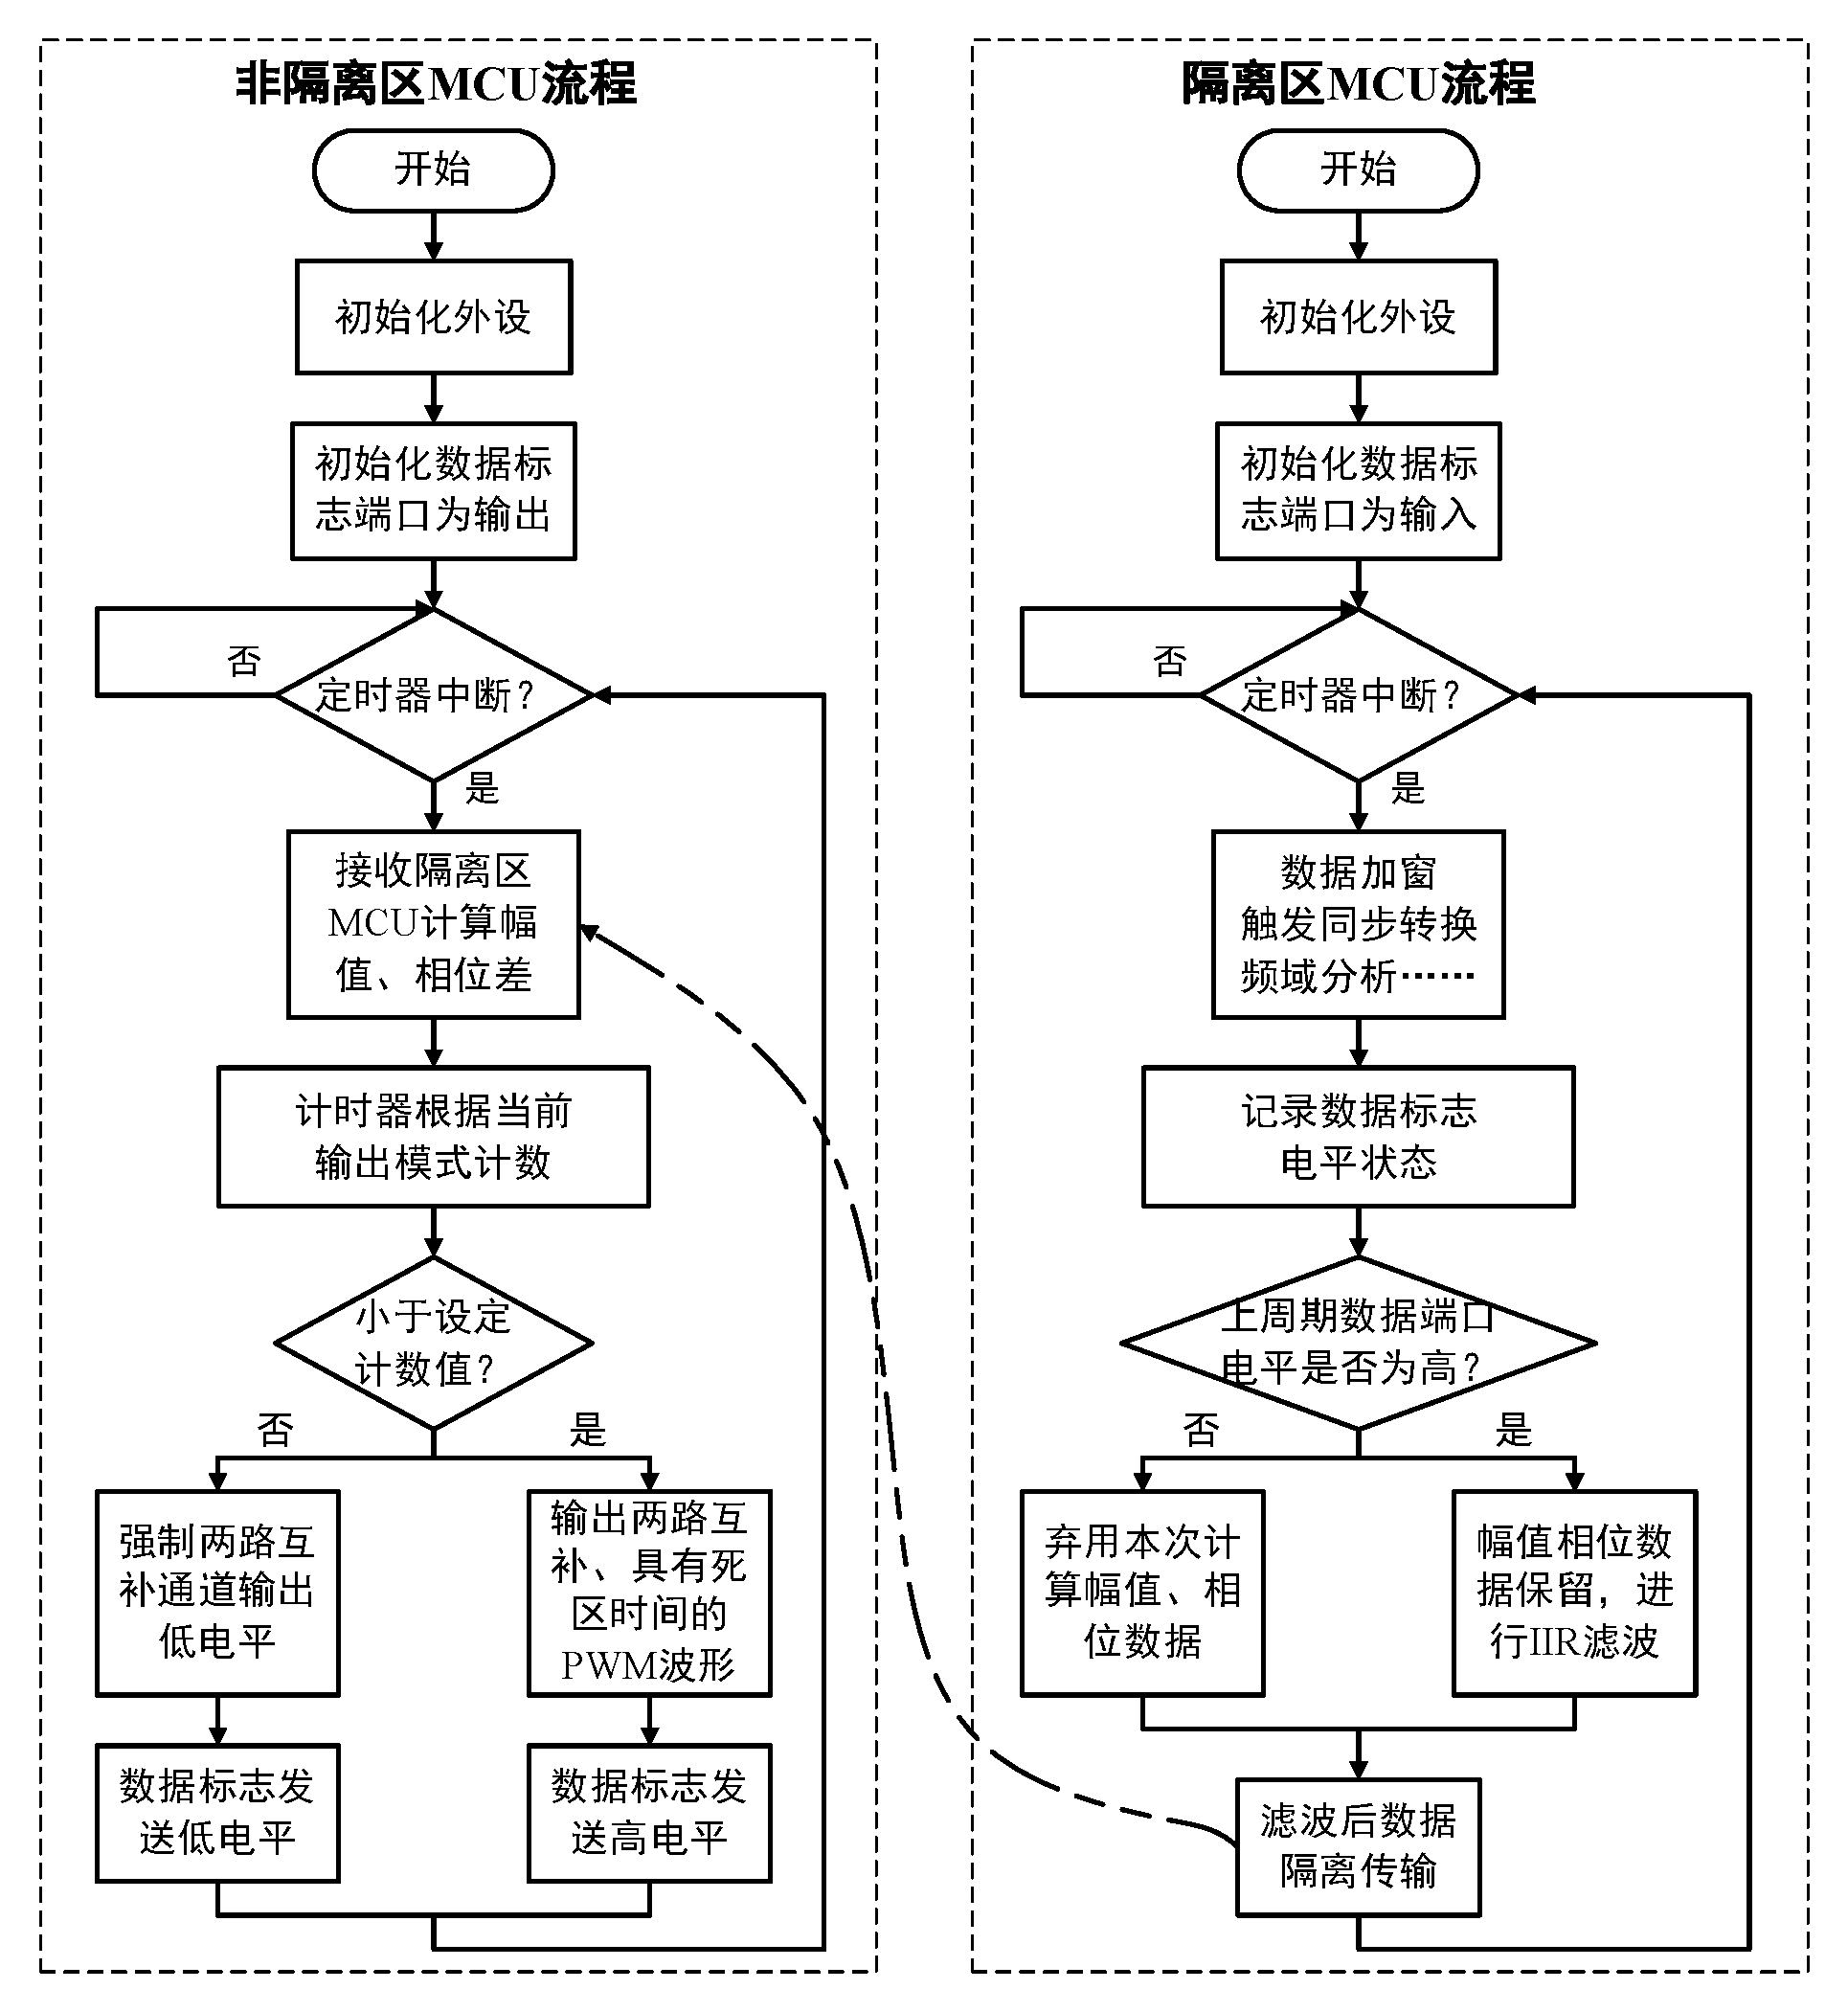
\includegraphics[scale=0.48]{Fig/cf_control.pdf}
	\caption{\label{cf_control}输出模式控制程序流程图}
\end{figure}

\subsection{有功功率控制}
在频域分析算法计算得到高频输出电压和电流的幅值以及相位差后，隔离区MCU依次对数据进行补偿、滤波以及输出拟合，然后通过隔离通信模块中的串口通道发送数据。非隔离区MCU在下一个控制周期接收后，可根据当前的输出模式计算出本控制周期内实际消耗在负载上的有功功率，作为控制器的反馈量。对LADRC功率控制器，其输入参考功率为使用者通过旋钮、按键等输入设备在人机交互系统设定，并通过SPI接口将数据传输到系统主板，控制器从而根据功率偏差计算出数字控制量。控制量通过SPI接口传输到可调直流源的DAC芯片中，经数模转换后其输出为降压稳压芯片的反馈引脚偏置电压，从而可以调整推挽逆变器输入的直流电压，进而调整系统的输出功率。

在功率控制过程中，系统需要实时监测输出电压和电流的幅值，若超出了设定的阈值则系统将切换为恒定电压控制或恒定电流控制，以改善高频输出信号在组织上的作用效果。此外，结合等效负载阻抗的计算，功率控制器不仅可以在设定功率变化下实时调整前馈补偿通道的比例系数，还可以根据阻抗的变化趋势对输出功率进行预测性调整，从而减小切割过程中的热损伤。

双核处理器同步架构下的有功功率控制流程图如图\ref{power_control}所示。
\begin{figure}[htbp]
	\centering
	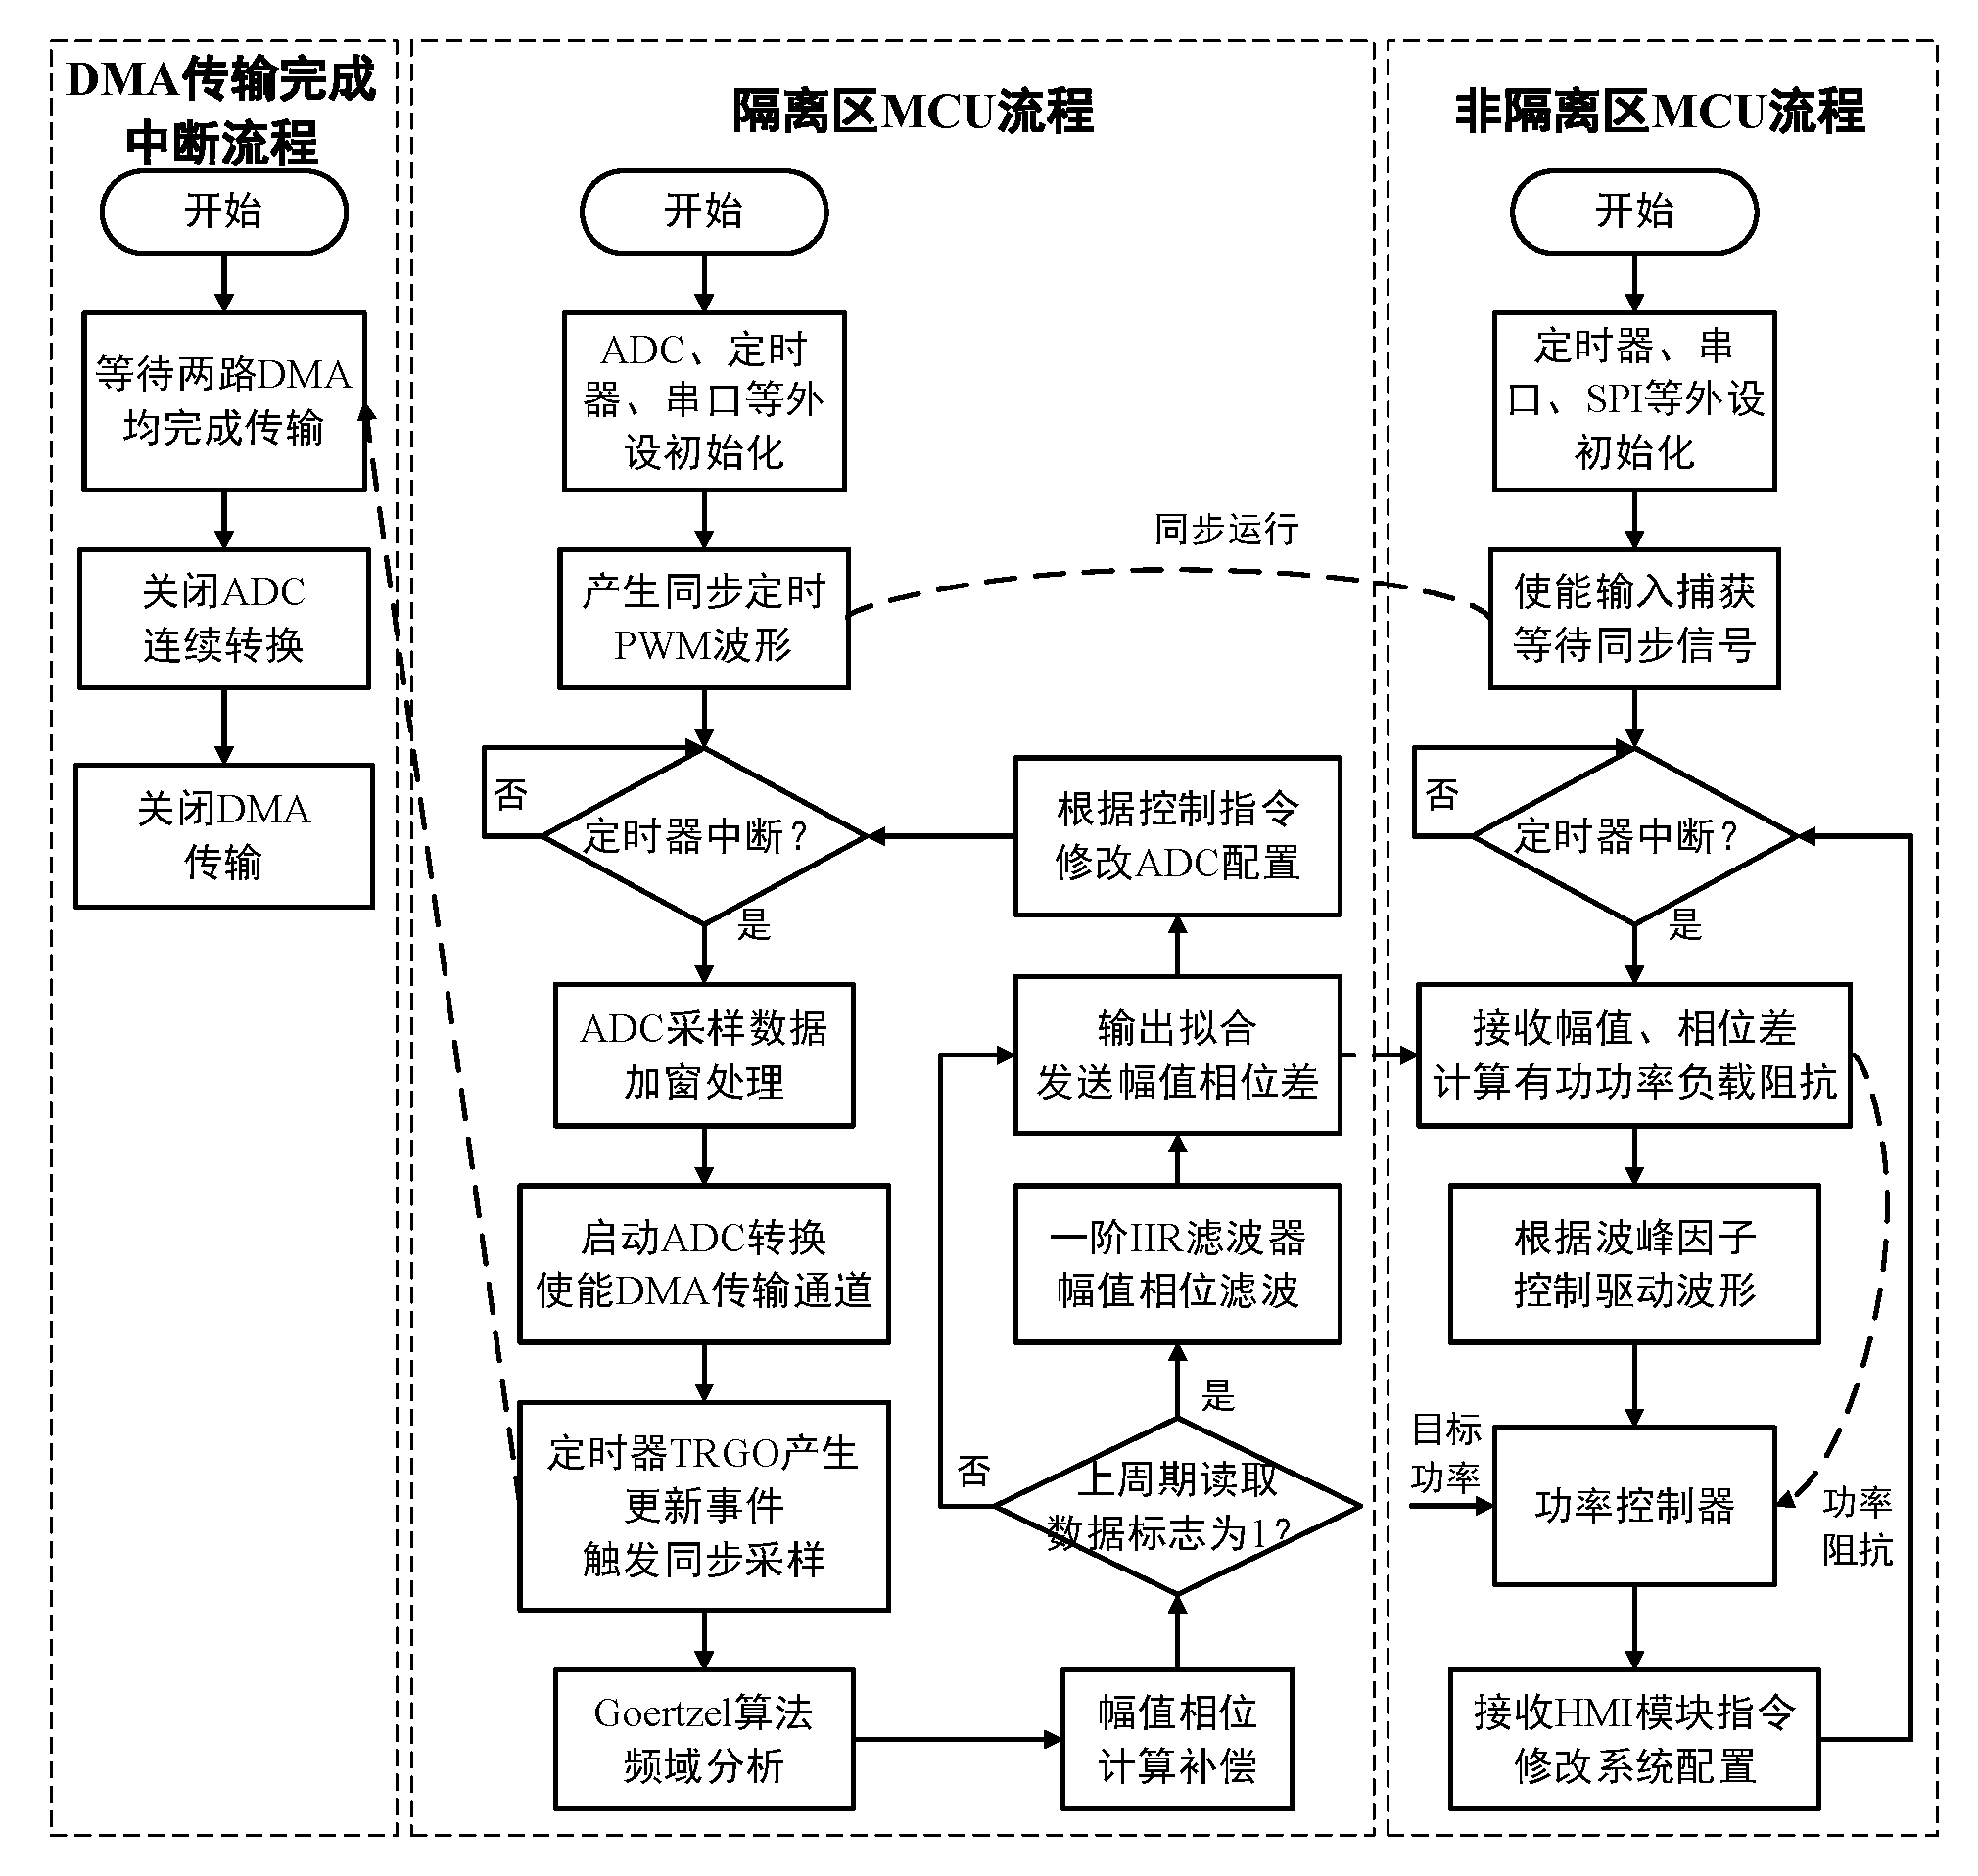
\includegraphics[scale=0.48]{Fig/power_control.pdf}
	\caption{\label{power_control}有功功率控制程序流程图}
\end{figure}


\section{人机交互系统软件设计}
基于3.6节设计的HMI板硬件资源，人机交互系统软件部分主要完成板载外设的驱动、功能逻辑的实现以及屏幕图形界面的设计。具体而言，外设驱动部分包括使用FSMC及IIC接口驱动触摸LCD显示屏、SDIO接口驱动SD卡、SPI接口驱动扩展Flash、定时器接口驱动旋钮编码器以及UART和DMA驱动主板通信模块；功能逻辑部分则在上述基本功能模块的基础上实现用户输入系统控制指令的处理、运行日志或字体资源等数据的存储与读取、与主板交互数据协议的填充和解析以及交互系统故障监测与处理等功能的处理逻辑，主要负责支撑人机交互系统的主要核心功能实现。

考虑到HMI板具有多种输入设备（旋钮、按键和触摸），且需要具有一定的美观性和易用性，本文在硬件资源充足的情况下选择使用LVGL图形库进行人机交互系统的屏幕图形界面设计。LVGL是一种采用C语言实现面向嵌入式系统的轻量级图形用户界面库，该图形库通过统一的显示、输入和时基接口与底层硬件相连接，实现界面绘制、交互响应与动画管理等功能。相较于直接使用底层LCD驱动进行界面开发，LVGL提供了大量控件和样式管理，降低了嵌入式图形界面设计与事件交互的复杂度。本文系统中LVGL设计的相关参数如表\ref{lvgl_param}所示。
\begin{table}[htbp]
	\caption{\label{lvgl_param}LVGL图形库设计参数}
	\centering
	\small
	\setlength{\tabcolsep}{20pt}
	\begin{tabular}{c c c c}
		\hline
		参数      & 数值      & 参数       & 数值    \\
		\hline
		显示分辨率   & 800×480 & 色彩深度     & 16bit \\
		屏幕刷新周期  & 30ms    & 输入设备数量   & 3     \\
		最大渲染堆空间 & 48KB    & DPI      & 130   \\
		输入设备数量  & 3       & 输入设备读取周期 & 30ms  \\
		LVGL版本  & 8.3.0   & 运行环境     & 裸机运行  \\
		\hline
	\end{tabular}
\end{table}

为进一步加速图形界面的开发，本文使用NXP推出的可视化前端设计工具GUI Guider进行界面设计，该工具通过拖拽方式完成界面布局、控件配置以及样式设计，并生成可直接集成到项目中的工程代码。本文设计的主要图形界面包含系统参数设定、状态显示以及菜单配置三个部分，其中系统参数设定用于用户输入系统的控制指令，如功率设定和模式选择等；状态显示用于实时显示系统的运行状态和工作参数；菜单配置用于提供系统的功能选项和设置界面。图形页面整体具有一致的设计风格和直观的交互体验，参数设定与菜单配置页面如图\ref{main_panel}和图\ref{settings_panel}所示。
\begin{figure}[htbp]
	\centering
	\begin{minipage}[c]{0.5\textwidth}
		\centering
		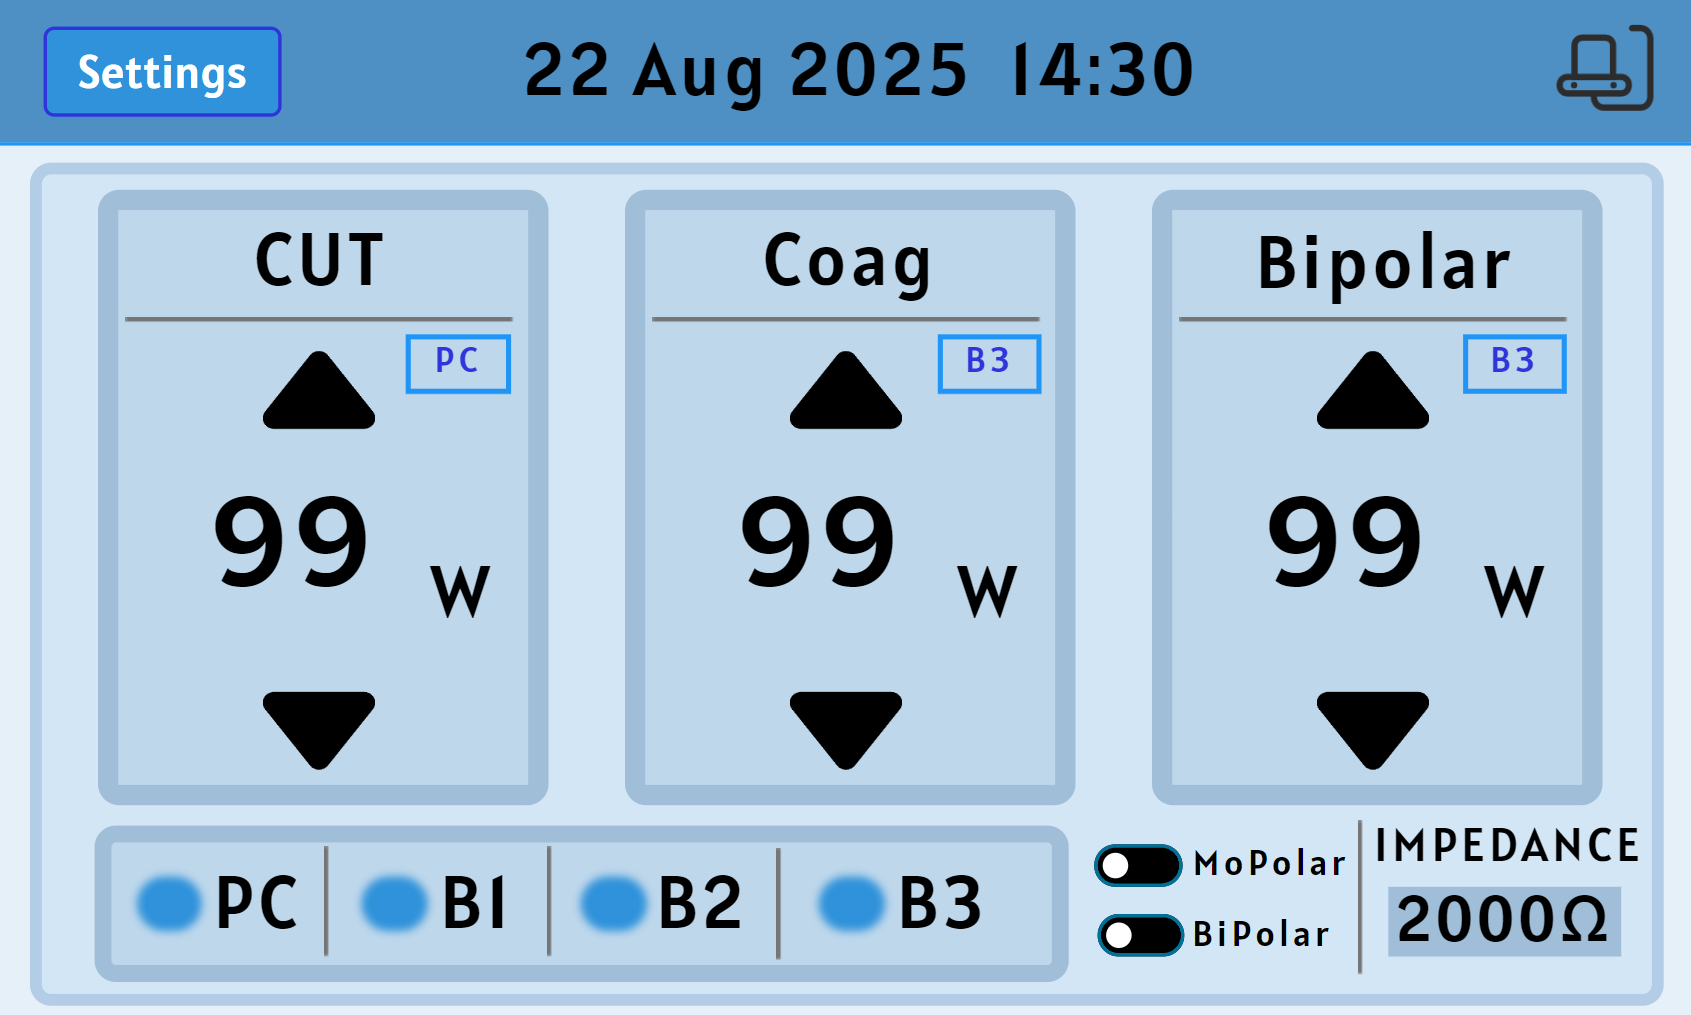
\includegraphics[scale=0.2]{Fig/main_panel.png} %1:1导入
	\end{minipage}%
	\begin{minipage}[c]{0.5\textwidth}
		\centering
		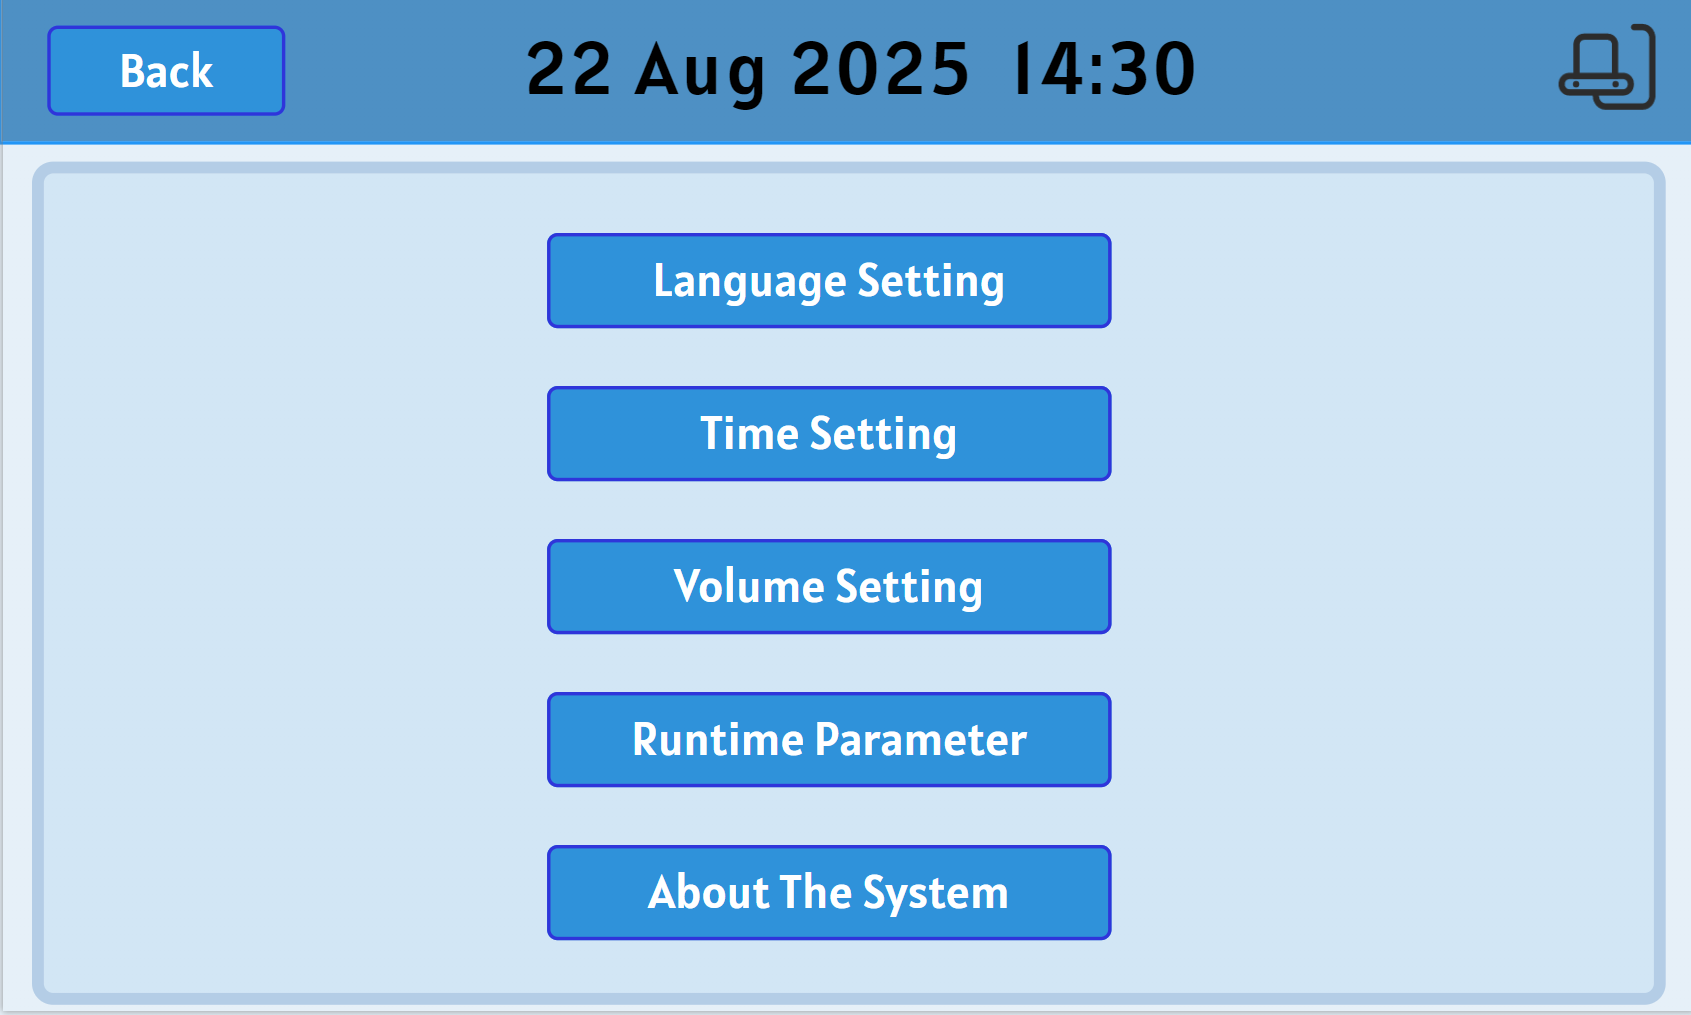
\includegraphics[scale=0.2]{Fig/settings_panel.png}
	\end{minipage}\\[1pt]
	\begin{minipage}[t]{0.5\textwidth} % 以下为新添加页面划分，[t]表示行顶部对齐
		\caption{\label{main_panel}首页参数设定界面}
	\end{minipage}%
	\begin{minipage}[t]{0.5\textwidth}
		\caption{\label{settings_panel}菜单配置界面}
	\end{minipage}%
\end{figure}

由上图可知，图形界面中包含了较多不同大小的字体以及图标等元素，GUI Guider通常会将这些资源文件输出为C数组格式，作为静态资源直接编译到项目工程中。当图形界面具有多种不同字体且图片较多时，静态编译的形式将会导致代码大小远超芯片存储资源的限制，从而此种方式限制了图形界面设计的灵活性。为此，本文将资源文件以binary格式存储到外部Flash或SD卡中，使用FatFs文件系统进行管理，在运行时通过LVGL的文件系统接口将FatFs挂载为逻辑文件驱动，从而使图形库能够以统一路径形式访问外部资源文件，有效降低了Flash空间的占用并便于资源替换和界面升级。

人机交互系统的程序流程图如图\ref{hmi_process}所示。
\begin{figure}[htbp]
	\centering
	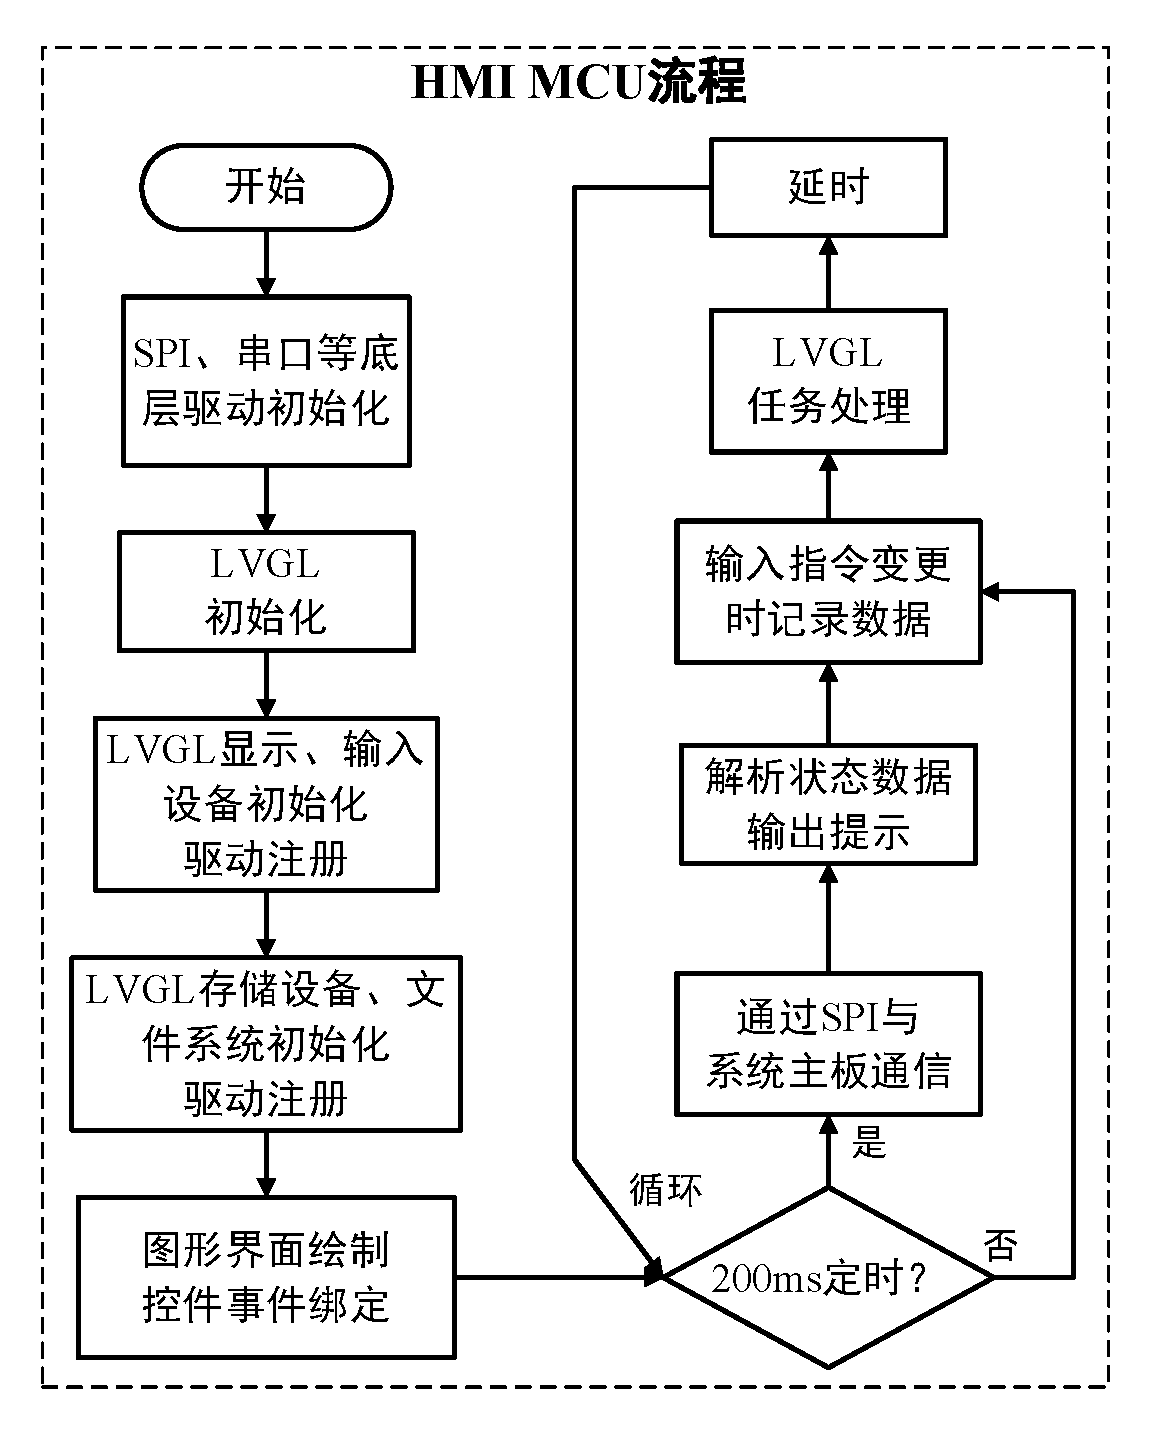
\includegraphics[scale=0.48]{Fig/hmi_process.pdf}
	\caption{\label{hmi_process}人机交互系统程序流程图}
\end{figure}

\section{本章小结}